\chapter{Los conceptos del Cálculo Integral}
\setcounter{chapter}{1}
\setcounter{section}{2}

\section{Funciones. Definición formal como conjunto de pares ordenados}
En cálculo elemental tiene interés considerar en primer lugar, aquellas funciones en las que el dominio y el recorrido son conjuntos de números reales. Estas funciones se llaman 
\textbf{Funciones de variable real} o funciones reales.\\

    \begin{tcolorbox}[colframe=white]
        %-----------------------------1.1. definición par ordenado-----------------------------
        \begin{def.}[Par ordenado]
            Dos pares ordenados $(a,b)$ y $(c,d)$ son iguales si y sólo si sus primeros elementos son iguales y sus segundos elementos son iguales.
            $$(a,b) = (c,d) \; \; \mbox{si y sólo si} \; \; a=c \; y \; b=d$$
        \end{def.}
    \end{tcolorbox}

    \begin{tcolorbox}[colframe=white]
        %----------------------------1.2 definición de función---------------------------------
        \begin{def.}[Definición de función]
            Una función $f$ es un conjunto de pares ordenados $(x,y)$ ninguno de los cuales tiene el mismo primero elemento.\\\\
            Debe cumplir las siguientes condiciones de existencia y unicidad:
            \begin{enumerate}[\bfseries (i)]
                \item $\forall x \in D_f, \exists y / (x,y) \in f(x) \; ó \; y=f(x)$
                \item $(x,y) \in  f \land (x,z) \in  f \Rightarrow y = z$
            \end{enumerate}
        \end{def.}
    \end{tcolorbox}

    \begin{tcolorbox}[colframe=white]
        %----------------------------1.3 definición dominio recorrido---------------------------
        \begin{def.}[Dominio y recorrido]
            Si $f$ es una función, el conjunto de todos los elementos $x$ que aparecen como primeros elementos de pares $(x,y)$ de $f$ se llama el \textbf{dominio} de $f$.  El conjunto de los segundos elementos y se denomina \textbf{recorrido} de $f$, o conjunto de valores de $f$.
        \end{def.}
    \end{tcolorbox}

        %----------------------teorema 1.1------------------------
        \begin{teo}
            Dos funciones $f$ y $g$ son iguales si y sólo si 
            \begin{enumerate}[\bfseries (a)]
                \item $f$ y $g$ tienen el mismo dominio, y
                \item $f(x) = g(x)$ para todo $x$ del dominio de $f.$\\
            \end{enumerate}
            Demostración.- \; Sea $f$ función tal que $x \in  D_f,\exists y \; / \; y=f(x)$ es decir $(x,f(x))$, $g$ una función talque $\forall  z \in  D_g , \exists  y \; / \; y=g(z)$ es decir $(z,g(z))$, entonces por definición de par ordenado tenemos que $(x,f(x)) = (z,g(z)) $ si y sólo si $x=z$ y $f(x)=g(z)$\\\\
        \end{teo}

    \begin{tcolorbox}[colframe=white]
        %--------------1.4 definición de sumas productos y cocientes de una función----------------------
        \begin{def.}[Sumas, productos y cocientes de funciones]
            Sean $f$ y $g$ dos funciones reales que tienen el mismo dominio $D$. Se puede construir nuevas funciones a partir de $f$ y $g$ por adición, multiplicación o división de sus valores. La función $u$ definida por,
            $$u(x) = f(x) + g(x) \; \; si \; x \in D$$
            se denomina suma de $f$ y $g$, se representa por $f+g.$ Del mismo modo, el producto $v=f cdot g$ y el cociente $w=f/g$ están definidos por las fórmulas
            $$v(x) = f(x) g(x) \; \; si \; x \in D, \; \; \, \, w(x) = f(x)/g(x) \; \; si \, x \, \in D \; y \; g(x) \neq 0$$
        \end{def.}
    \end{tcolorbox}
    
\setcounter{section}{4}
\section{Ejercicios}
    \begin{enumerate}[\Large \bfseries 1.]
        %--------------------1.-------------------
        \item Sea $f(x)=x+1$ para todo real $x$. Calcular:
            \begin{itemize}
                \item $f(2) = 2+1 = 3$\\\\
                \item $f(-2) = -2 +1 = -1$\\\\
                \item $-f(2) = -(2+1)=-3$\\\\
                \item $f \left( \dfrac{1}{2} \right) = \dfrac{1}{2} + 1 = \dfrac{3}{2}$\\\\
                \item $\dfrac{1}{f(2)}= \dfrac{1}{3}$\\\\
                \item $f(a+b) = a+b+1$\\\\
                \item $f(a)+f(b)= (a+1) + (b+1) = a+b+2$\\\\
                \item $f(a) \cdot f(b) = (a+1)(b+1) = ab + a + b + 1$\\\\
            \end{itemize}

        %--------------------2.--------------------
        \item Sean $f(x)= 1+x$ \; y \; $g(x)=1-x$ para todo real $x$. calcular:
            \begin{itemize}
                \item $f(2)+g(2) = (1+2) + (1-2) = 2$\\\\
                \item $f(2)-g(2) = (1+2) - (1-2) = 4$\\\\
                \item $f(2)\cdot g(2) = (1+2) \cdot (1-2) = 3 \cdot (-1) = -3$\\\\
                \item $\dfrac{f(2)}{g(2)}= \dfrac{1+2}{1-2} = \dfrac{3}{-1} = -3$\\\\
                \item $f\left[ g(2)\right] = f(1-2) = f(-1) = 1+(-1)= 0$\\\\
                \item $g\left[ f(2)\right] = f(1+2) = g(3) = 1 - 3 = -2$\\\\
                \item $f(a) + g(-a) = (1+a) + (1 - a) = 2$\\\\
                \item $f(t)\cdot g(-t) = (1+t) \cdot (1+t) = 1 + t + t + t^2 = t^2 +2t + 1 = (t+1)^2$\\\\
            \end{itemize}
        
        %--------------------3.---------------------
        \item Sea $f(x)=|x-3|+|x-1|$ para todo real $x$. Calcular:\\
            \begin{itemize}
                \item $f(0) = |0-3|+|0-1| = 3 + 1 = 4$
                \item $f(1) = |1-3|+|1-1| = 2$
                \item $f(2) = |2-3|+|2-1| = -1 + 1 = 2$
                \item $f(3) = |3-3|+|3-1| = 2$
                \item $f(-1) = |-1-3|+|-1-1| = 4 + 2 = 6$
                \item $f(-2) = |-2-3|+|-2-1| = 5 + 3 = 8$\\
            \end{itemize}
            Determinar todos los valores de $t$ para los que $f(t+2)=f(t)$\\
            \begin{center}
                \begin{tabular}{r c l}
                    $|t+2-3| + |t+2-1|$&=&$|t-3| + |t-1|$\\
                    $|t-1|+|t+1|$&=&$|t-3|+|t-1|$\\
                    $|t+1|$&=&$t-3$\\
                \end{tabular}
            \end{center}
            Por lo tanto  $t=1$\\\\

        %--------------------4.-------------------
        \item Sea $f(x)=x^2$  para todo real $x$. Calcular cada una de las fórmulas siguientes. En cada caso precisar los conjuntos de números erales $x, \; y \; t,$ etc., para los que la fórmula dada es válida.
            \begin{enumerate}[\bfseries (a)]
                %----------(a)----------
                \item $f(-x)=f(x)$ \\\\
                Demostración.- \; Se tiene $f(-x) = (-x)^2 = x^2 = f(x) \; \forall x \in \mathbb{R}$\\\\

                %----------(b)----------
                \item $f(y)-f(x)=(y-x)(y+x)$\\\\
                Demostración.- \; $f(y)-f(x)= y^2 - x^2 = (x-y)(x+y), \; \forall x, \; y \in \mathbb{R}$\\\\

                %----------(c)----------
                \item $f(x+h) - f(x) = 2xh + h^2$\\\\
                Demostración.- \; $f(x+h) - f(x) = (x+h)^2 -x^2 = x^2 + 2xh +h^2 - x^2 = 2xh + h^2, \; \forall x \in \mathbb{R}$\\\\

                %----------(d)----------
                \item $f(2y) = 4f(y)$\\\\
                Demostración.- \; $f(2y) = (2y)^2 = 4y^2 = 4 f(y), \; \forall y \in \mathbb{R}$\\\\
                %----------(e)----------
                \item $f(t^2)=f(t)^2$\\\\
                Demostración.- \; $f(t^2) = (t^2)^2 = f(t)^2$\\\\
                %----------(f)----------
                \item $\sqrt{f(a)} = |a|$\\\\
                Demostración.- \; $\sqrt{f(a)} = \sqrt{a^2} = |a|$\\\\
            \end{enumerate}

        %--------------------5.--------------------
        \item Sea $g(x) = \sqrt{4-x^2}$ para $|x| \leq 2$. Comprobar cada una de las fórmulas siguientes e indicar para qué valores de $x, \; y, s$ y $t$ son válidas.
            \begin{enumerate}[\bfseries (a)]
                %----------(a)----------
                \item $g(-x) = g(x)$\\\\
                Se tiene $g(-x)=\sqrt{2-(-x)^2} = \sqrt{2-(x)^2} = g(x), \; \; para \; |x| \leq 2$\\\\

                %----------(b)----------
                \item $g(2y) = 2\sqrt{1-y^2}$\\\\
                $g(2y)=\sqrt{4-(2y)^2}= \sqrt{4(1-y^2)} = 2 \sqrt{1-y^2}, \; \; para \; |y|\leq 1$ Se obtiene $|y| \leq 1$  de $\sqrt{1-y^2}$ es decir $1-y^2 \geq 0$ entonces $\sqrt{y^2} \leq \sqrt{1}$ \; y \; $|y|\leq 1$\\\\

                %----------(c)----------
                \item $g\left( \dfrac{1}{t} \right) = \dfrac{\sqrt{4t^2-1}}{|t|}$\\\\
                $g\left( \dfrac{1}{t} \right) = \sqrt{4 - \left( \dfrac{1}{t} \right)^2} = \sqrt{\dfrac{4t^2 - 1}{t^2}} =\dfrac{\sqrt{4t^2 - 1}}{|t|}, \; \; para \; |t| \geq \dfrac{1}{2}$\\\\
                Para hallar los valores correspondientes debemos analizar $\sqrt{4t^2 - 1}$. Es decir $$4t^2-1 \geq 0 \Rightarrow 4t^2 \geq 1 \Rightarrow t^2 \geq \dfrac{1}{2^2} \Rightarrow |t| \geq \dfrac{1}{2}$$\\

                %----------(d)----------
                \item $g(a-2) = \sqrt{4a-a^2}$\\\\
                $g(a-2) = \sqrt{4 - x^2} = \sqrt{4 - (a-2)^2} = \sqrt{4a - a^2}, \; \; para \; 0\leq a \leq 4.$ Basta probar  $4a-a^2 \geq 0$\\\\

                %----------(e)----------
                \item $g \left( \dfrac{s}{2} \right) = \dfrac{1}{2} \sqrt{16 - s^2}$\\\\
                $s\left( \dfrac{s}{2} \right) = \sqrt{4 - \left( \dfrac{s}{2} \right)^2} = \dfrac{\sqrt{16 - s^2}}{2}, \; \; para \; |s| \leq 4$. ya que solo basta comprobar que $\sqrt{16 - s^2} \geq 0$\\\\

                %----------(f)----------
                \item $\dfrac{1}{2 +g(x)} = \dfrac{2-g(x)}{x^2}$\\\\ 
                $\dfrac{1}{2 +g(x)} = \dfrac{1}{2+ \sqrt{4-x^2}} \cdot \dfrac{2 - \sqrt{4-x^2}}{2 - \sqrt{4-x^2}} = \dfrac{2 - g(x)}{x^2}\; para \; \; |x| \leq 2 \; y \; x \neq 0$\\\\ 
                Evaluemos $\sqrt{4-x^2}$. Sea $4-x^2 \geq 0$ entonce $\sqrt{x^2} \leq 2$. Por otro lado tenemos que la función no puede ser $0$ por $\dfrac{1}{x^2}$, por lo tanto debe ser $x^2\neq 0$.\\\\ 
            \end{enumerate}

        %--------------------6.-------------------
        \item Sea $f$ la función definida como sigue: $f(x)=1$ para $0 \leq x \leq 1;$ $f(x)=2$ para $1 < x \leq 2$. La función no está definida si $x<0$ ó si $x >2.$
            \begin{enumerate}[\bfseries (a)]
                %----------(a)----------
                \item Trazar la gráfica de $f$ 
                    \begin{center}
                        \begin{tikzpicture}[scale=1,draw opacity = 0.6]
                            % abscisa y ordenada
                            \tkzInit[xmax= 3,xmin=0,ymax=3,ymin=0]
                            \tiny\tkzLabelXY[opacity=0.6,step=1, orig=false]
                            % etiqueta x, f(x)
                            \tkzDrawX[opacity=0.6,label=x,right=0.3]
                            \tkzDrawY[opacity=0.6,label=f(x),below = -0.6]
                            %dominio y función
                            \draw [domain=0:1,thick,gray] plot(\x,{1});
                            \tkzText[opacity=0.6,above](0.5,1){\tiny $f(x)=1$}
                            \draw [domain=1:2,thick,gray] plot(\x,{2});
                            \tkzText[opacity=0.6,above](1.5,2){\tiny $f(x)=2$}
                            % intervalos
                            \draw[fill=black] (0,1) circle (1.5pt);
                            \draw[fill=black] (1,1) circle (1.5pt);
                            \draw[          ] (1,2) circle (1.5pt);
                            \draw[fill=black] (2,2) circle (1.5pt);
                        \end{tikzpicture}
                    \end{center}

                %----------(b)----------
                \item Poner $g(x) = f(2x).$ Describir el dominio de $g$ y dibujar su gráfica.
                    \begin{center}
                        \begin{tikzpicture}[scale=1,draw opacity = 0.6]
                            % abscisa y ordenada
                            \tkzInit[xmax= 3,xmin=0,ymax=3,ymin=0]
                            \tiny\tkzLabelXY[opacity=0.6,step=1, orig=false]
                            % label x, f(x)
                            \tkzDrawX[opacity=0.6,label=x,right=0.3]
                            \tkzDrawY[opacity=0.6,label=f(x),below = -0.6]
                            %dominio y función
                            \tkzFct[opacity=1,domain = 0:0.5]{1}
                            \draw [domain=0:0.5,thick,gray] plot(\x,{1}); 
                            \tkzFct[opacity=1,domain = 0.5:1]{2} 
                            % intervalos
                            \tkzSetUpPoint[shape=circle, size = 3, color=black, fill=black]
                            \tkzDefPointByFct[draw,with = a](0)
                            \tkzDefPointByFct[draw,with = a](0.5)
                            \tkzDefPointByFct[draw,with = b](1)
                            \tkzSetUpPoint[shape=circle, size = 3, color=black, fill=white]
                            \tkzDefPointByFct[draw,with = b](0.5)
                        \end{tikzpicture}
                    \end{center}
                Debido a que $1\leq 2x \leq 1$ \; y \; $1 < 2x \leq 2$ el dominio de $g(x)$ es $0\leq x \leq 1$\\\\ 

                %----------(c)----------
                \item Poner $h(x) = f(x-2).$ Describir el dominio de $k$ \; y dibujar su gráfica.
                    \begin{center}
                        \begin{tikzpicture}[scale=1,draw opacity = 0.6]
                            % abscisa y ordenada
                            \tkzInit[xmax= 4,xmin=0,ymax=3,ymin=0]
                            \tiny\tkzLabelXY[opacity=0.6,step=1, orig=false]
                            % label x, f(x)
                            \tkzDrawX[opacity=0.6,label=x,right=0.3]
                            \tkzDrawY[opacity=0.6,label=f(x),below = -0.6]
                            %dominio y función
                            \tkzFct[opacity=1,domain = 2:3]{1} 
                            \tkzFct[opacity=1,domain = 3:4]{2} 
                            % intervalos
                            \tkzSetUpPoint[shape=circle, size = 3, color=black, fill=black]
                            \tkzDefPointByFct[draw,with = a](2)
                            \tkzDefPointByFct[draw,with = a](3)
                            \tkzDefPointByFct[draw,with = b](4)
                            \tkzSetUpPoint[shape=circle, size = 3, color=black, fill=white]
                            \tkzDefPointByFct[draw,with = b](3)
                        \end{tikzpicture}
                    \end{center}
                Debido a que $1\leq x-2 \leq 1$ \; y \; $1 < x-2 \leq 2$ el dominio de $h(x)$ es $2\leq x \leq 4$\\\\ 

                %----------(d)----------
                \item Poner $k(x) = f(2x) + f(x-2).$ Describir el dominio de $k$ \; y dibujar su gráfica.\\\\
                El dominio está vacío ya $f(2x)$ que solo está definido para $0 \leq x \leq 1$ \; y \;  $f(x-2)$ solo está definido para $2 \leq x \leq 4$. Por lo tanto no hay ninguno $x$ que satisfaga ambas condiciones. \\\\
            \end{enumerate}
        
        %--------------------7.-------------------
        \item Las gráficas de los dos polinomios $g(x)=x$ \; y \; $f(x)=x^3$ se cortan en tres puntos. Dibujar una parte suficiente de sus gráficas para ver cómo se cortan.
            \begin{center}
                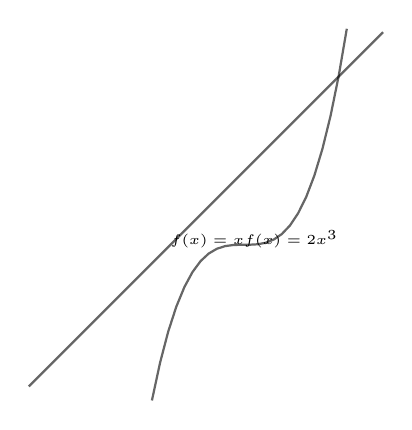
\begin{tikzpicture}[scale=0.9, draw opacity = .6]
                    % abscisa y ordenada
                    \tkzInit[xmax= 3,xmin=-2,ymax=3,ymin=-2]
                    \tiny\tkzLabelXY[opacity=0.6,step=1, orig=false]
                    % label x, f(x)
                    \tkzDrawX[opacity= .6,label=x,right=0.3]
                    \tkzDrawY[opacity= .6,label=f(x),below = -0.6]
                    %dominio y función
                    \draw [domain=-2:3,thick] plot(\x,{\x}); 
                    \tkzText[above,opacity=0.6](3.3,3){\tiny $f(x)=x$}
                    \draw [domain=-1.3:1.45,thick] plot(\x,{\x^3}); 
                    \tkzText[above,opacity=0.6](1.2,3){\tiny $f(x)=2x^3$}
                \end{tikzpicture}
            \end{center}  

        %--------------------8.-------------------
        \item Las gráficas de los dos polinomios cuadráticos $f(x) = x^2-2$ \; y \; $g(x)=2x^2+4x+1$ se cortan en dos puntos. Dibujar las porciones de sus gráficas comprendidas entre sus intersecciones.
            \begin{center}
                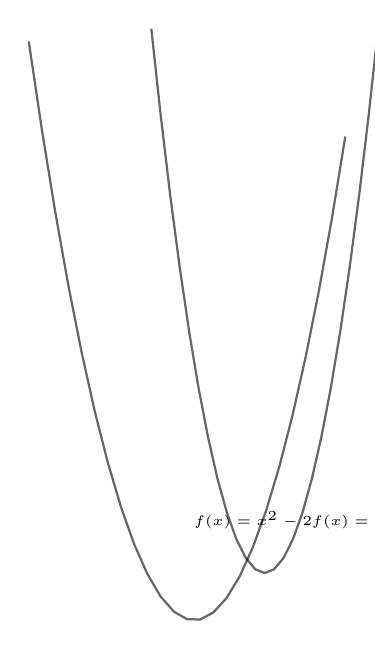
\begin{tikzpicture}[scale=.6, draw opacity = .6]
                    % abscisa y ordenada
                    \tkzInit[xmax= 4,xmin=-4,ymax=10,ymin=-3]
                    \tiny\tkzLabelXY[opacity=0.6,step=1, orig=false]
                    % label x, f(x)
                    \tkzDrawX[opacity= .6,label=x,right=0.3]
                    \tkzDrawY[opacity= .6,label=f(x),below = -0.6]
                    %dominio y función
                    \draw [domain=-3.5:3.2,thick] plot(\x,{\x*\x - 2});  
                    \tkzText[above,opacity=0.6](4,8.2){\tiny $f(x)=x^2 - 2$}
                    \draw [domain=-3.4:1.4,thick] plot(\x,{2*\x*\x + 4*\x + 1});  
                    \tkzText[above,opacity=0.6](3,10.5){\tiny $f(x)=2x^2 +4x + 1$}
                \end{tikzpicture}
            \end{center} 

        %--------------------9.-------------------
        \item Este ejercicio desarrolla ciertas propiedades fundamentales de los polinomios. Sea $f(x)=\displaystyle\sum_{k=0}^{n} c_k x^k$ un polinomio de grado $n$. Demostrar cada uno de los siguientes apartados:
            \begin{enumerate}[\bfseries (a)]
                %----------(a)----------
                \item Si $n \geq 1$ \; y \; $f(0)=0,$ $f(x)=xg(x)$, siendo $g$ un polinomio de grado $n-1.$\\\\
                Para entender lo que nos quiere decir Apostol pongamos un ejemplo. Supongamos que tenemos un polinomio donde $f(x)=2x^2+3x-x$ entonces notamos que $f(x)=x(2x+3-1)$ donde $g(x)=2x+3-1$, esto quiere decir que si $0 = f(0)=c_0 \Rightarrow c_1 x + c_2 x^2 + ... + c_n x^n = x(c_1 + c_2 x + ... + c_n x^{n-1})$ 
                Así que debemos demostrar que $f(x)$ es un polinomio arbitrario de grado $n \geq 1$ tal que $f(0)=0$, entonces debe haber un polinomio de grado $n-1, \; g(x)$, tal que $f(x)=xg(x)$\\\\
                Demostración.- \; Sabemos que $$f(0) = c_n \cdot 0^n + c_{n-1} \cdot 0^{n-1} + ... + c_1 \cdot 0 + c_0 =c_0,$$ como $f(0)=0$ se concluye que $c_0=0$. Así tenemos $$f(x)=\displaystyle\sum_{k=1}^{n} c_k x^k.$$ Ahora crearemos una función $g(x).$ Dada la función $f(x)$ como la anterior, definamos, $$f(x)=\displaystyle\sum_{k=0}^{n} c_k x^{k-1} = \sum_{k=1}^{n} c_k x^{k-1}$$ 
                Ahora crearé una función $g(x)$. Dada una función $f(x)$ como la anterior, definamos  $$g(x) = \displaystyle\sum_{k=1}^{n} c_k x^{k-1}$$
                donde $c_k$ son los mismos que los dados por la función $f(x)$. Primero notemos que el grado de $g(x)$ es $n-1$. Finalmente, tenemos que $$ xg(x) = x \displaystyle\sum_{k=1}^{n} c_k x^{k-1} = \sum_{k=1}^{n} c_k x^k = f(x).$$ \\\\

                %----------(b)----------
                \item Para cada real $a$, la función $p$ dada por $p(x)=f(x+a)$ es un polinomio de grado $n.$\\\\
                Demostración.- \; Usando el teorema del binomio,
                    \begin{center}
                        \begin{tabular}{r c l}
                            $f(x+a)$&=&$ \displaystyle\sum_{k=0}^{n} (x+a)^k c_k$\\\\
                            &=&$c_o + (x+a)c_1 + (x+a)^2 c_2 + ...+(x+a)^n c_n$\\\\
                            &=&$ c_o + c_1 \left( \displaystyle\sum_{j=0}^{1} {1 \choose j} a^j x^{1-j} \right) + c_2 \left( \displaystyle\sum_{j=0}^2 {2 \choose j} a^j x^{2-j} \right) 
                            + ... + c_n \left( \displaystyle\sum_{j=0}^{n} {n \choose j} a^j x^{n-j} \right)$\\\\
                            &=&$(c_o + ac_1 + a^2 c_2 + ... + a^n c_n) + x(c_1 + 2ac_2 + ... + na^{n-1} c_n)$\\\\
                            &=&$\displaystyle\sum_{k=0}^n \left( x^k \left( \displaystyle\sum_{j=k} {j \choose j-k} c_j a{j-k}\right) \right)$\\
                        \end{tabular}
                    \end{center}
                En la linea final reescribimos los coeficientes como sumas para verlos de manera más concisa. De cualquier manera, dado que todos los $c_i$ son constantes, tenemos $\displaystyle\sum_{j=k}^n {j \choose j-k} c_j a^{j-k}$ es alguna constante para cada $k,$ de $d_k$ y tenemos, $$p(x) = \displaystyle\sum_{k=0}^n d_k x^k$$\\\\

                %----------(c)----------
                \item Si $n \geq 1$ \; y \; $f(a)=0$ para un cierto valor real $a$, entonces $f(x) = (x-a) \, h(x),$ siendo $h$ un polinomio de grado $n-1$. (considérese $p(x)=f(x+a).$)\\\\
                Demostración.- \; Por la parte $b)$ se sabe que $f(x)$ es un polinomio de grado $n$, entonces $p(x)=f(x+a)$ también es un polinomio del mismo grado. Ahora si $f(a)=0$ entonces por hipótesis $p(0)=f(a)=0$. Luego por la parte $a)$, tenemos $$p(x)=x \cdot g(x)$$ donde $g(x)$ es un polinomio de grado $n-1$. Así,
                $$p(x-a)=f(x)= f(x) = (x-a) \cdot g(x-a)$$ ya que $p(x)=f(x+a)$. Pero, si $g(x)$ es un polinomio de grado $n-1$, entonces por la parte $b)$ nuevamente, también lo es $h(x)=g(x+(-a)) = g(x-a)$. Por lo tanto, $$f(x)=(x-a) \cdot h(x)$$ para $h$ un grado $n-1$ polinomial, según lo solicitado.\\\\\

                %----------(d)----------
                \item Si $f(x)=0$ para $n+1$ valores reales de $x$ distintos, todos los coeficientes $c_k$ son cero y $f(x)=0$ para todo real de $x$\\\\
                Demostración.- \;  La prueba se realizara por inducción. Sea $n=1$, entonces $f(x)=c_o + c_1 x$. Dado que la hipótesis es que existen $n+1$ distintos  $x$ de tal manera que $f(x)=0$, sabemos que existen $a_1$, $a_2$ $\in \mathbb{R}$ tal que $$f(a_1)=f(a_2)=0, \; \; \; a_1 \neq a_2,$$ Así, 
                    \begin{center}
                        \begin{tabular}{r c l c r c l l}
                            $c_0 + c_1 a_1$&$=$&$0$&$\Rightarrow$&$c_1 a_1 - c_1 a_2$&$=$&$0$&\\
                            &&&$\Rightarrow$&$c_1(a_1 - a_2)$&$=$&$0$&\\
                            &&&$\Rightarrow$&$c_1$&$=$&$0$& ya que $a_1 \neq a_2$\\
                            &&&$\Rightarrow$&$c_0$&$=$&$0$&ya que $c_0 + c_1 a_1 = 0$\\
                        \end{tabular}
                    \end{center}
                Por lo tanto, la afirmación es verdadera. Suponga que es cierto para algunos $n=k \in \mathbb{Z}^{+}$. Luego Sea $f(x)$ un polinomio de grado $k+1$ con $k+2$ distintos de $0$, $a_1,...,a_{k+2}.$ ya que $f(a_{k+2}) = 0$, usando la parte $c)$, tenemos, $$f(x)=(x- a_{k+2})h(x)$$
                donde $h(x)$ es un polinomio de grado $k$. Sabemos que hay $k+1$ valores distintos $a_1,... a_{k+1}$ tal que  $h(a_i) = 0.$ Dado que $f(a_i)=0$ para $1< i < k+2y$ y $(x- a_{k+2}) \neq 0$ para $x=a_i$ con $1 < i < k+1$ ya que todos los $a_1$ son distintos), por lo tanto, según la hipótesis de inducción, cada coeficiente de $h$ es $0$ y $h(x)=0$ para todo $x \in \mathbb{R}.$ Así,
                    \begin{center}
                        \begin{tabular}{r c r c l}
                            $f(x)$&$=$&$(x - a_{k+2})h(x)$&$=$&$(x- a_{k+2}) \cdot \displaystyle\sum_{j=0}^k c_j x^j$\\\\
                            &&&$=$&$\displaystyle\sum_{j=0}^k (x - a_{k+2})c_j x^j$\\\\
                            &&&$=$&$c_k x^{k+1} + (c_{k-1} - a_k + 2c_k)x^k + ... + (c_1 -a_{k+2} c_0)x + a_{k+2} c_0$\\
                        \end{tabular}
                    \end{center}
                Pero dado que todos los coeficientes de $h(x)$ son cero y $f(x) = 0$ para todo $x \in \mathbb{R}$. Por lo tanto, la afirmación es verdadera para el caso $k+1$ y para todo $n \in \mathbb{Z}^+$\\\\

                %----------(e)----------
                \item Sea $g(x) = \displaystyle\sum_{k=0}^m b_k x^k$ un polinomio de grado $m$, siendo $m \geq n.$ Si $g(x)=f(x),$ para $m+1$ valores reales de $x$ distintos, entonces $m=n$, $b_k =c_k$ para cada valor de $k$, y $g(x)=f(x)$ para todo real $x$\\\\
                Demostración.- \; Sea $$p(x)=g(x)-f(x) = \displaystyle\sum_{k=0}^m b_k x^k - \sum_{k=0}^n c_k x^k = \sum_{k=0}^m (b_k - c_k)x^k$$ donde $c_k=0$ para $n< k \leq m$, cabe recordar que tenemos $m \geq n$.\\
                Entonces, hay $m+1$ distintos reales $x$ para los cuales $p(x)=0$. Dado que hay $m+1$ valores reales distintos para lo cuál $g(x)=f(x),$ así en cada uno de estos valores $p(x)=g(x)-f(x)=0$. Por lo tanto, por la parte $d)$, $b_k-c_k =0$ para $k=0,...,m$ y $p(x)=0$ para todo $x \in \mathbb{R}$. Es decir $$b_k - c_k =0 \; \; \; \Rightarrow \; \; \; b_k=c_k \; \; \; para \; k=0,...,m$$ y $$p(x)=0 \; \; \; \Rightarrow \; \; \; g(x)-f(x)=0 \; \; \; \Rightarrow \; \; \; f(x)=g(x),$$ para todo $x \in \mathbb{R}$. Ademas desde $b_k -c_k =0$ para $k=0,..., m$ y por supuesto $c_k=0$ para $k=n+1, ... , m,$ tenemos $b_k=0$ para $k= n+1, ... , m.$ Pero entonces, $$g(x)=\displaystyle\sum_{k=0}^n b_k x^k + \sum_{k=n+1}^m 0 \cdot x^k = \sum_{k=0}^n b^k x^k$$ significa que $g(x)$ es un polinomio de grado $n$ también.\\\\

            \end{enumerate}

        %--------------------10.-------------------
        \item En cada caso, hallar todos los polinomios $p$ de grado $\leq 2$ que satisfacen las condiciones dadas.\\\\
        Sabemos que para un polinomio de grado $\leq 2$ es:
        $$p(x) = ax^2 + bx + c$$ 
        para todo $a,b,c \in \mathbb{R}$.\\\\
            \begin{enumerate}[\bfseries (a)]
                %----------(a)-----------
                \item $p(x) = p(1-x)$\\\\
                Sea $f(x) = p(x) -1$, entonces $f$ es de grado como máximo $2$ por la parte $d)$ del problema $9$ tenemos que  todos los coeficientes de $f$ son $0$ \; y \; $f(x)=0$ para todo $x \in \mathbb{R}$, así,
                $$p(x)-1 = 0 \; \; \Rightarrow \; \; p(x)=1 \; \; \forall x \in \mathbb{R}$$\\\\ 

                %----------(b)-----------
                \item $p(x) = p(1+x)$\\\\
                Tenemos $p(0)=1 \Rightarrow c=1$ luego, $p(1)=1 \Rightarrow a+b=0 \Rightarrow b=-a$ y finalmente, con $c=1$ \; y \; $b=-a$, tenemos: $p(2)=2 \Rightarrow 4a-2a=1 \Rightarrow a=\dfrac{1}{2}, \; b=-\dfrac{1}{2}$. por lo tanto $$p(x)=\dfrac{1}{2}x^2 - \dfrac{1}{2}x + 1 = \dfrac{1}{2}x(x-1) + 1$$\\\\

                %----------(c)-----------
                \item $p(x) = p(0) = p(1) =1$\\\\
                Una vez mas, desde $p(0)=1$ tenemos: $a+b=0 \Rightarrow b=-a$ así, $p(x) = ax^2 - ax + 1 = ax(x-1) + 1$\\\\

                %----------(d)-----------
                \item $p(0) = p(1)$\\\\
                Simplemente sustituyendo estos valores que tenemos, $p(0)=p(1) \Rightarrow c=a+b+c \Rightarrow b=-a$ entonces, $$p(x) = ax^2 -ax + c = ax(x-1) + c$$\\\\

            \end{enumerate}
            
        %--------------------11.-------------------
        \item En cada caso, hallar todos los polinomios $p$ de grado $\leq 2$ que para todo real $x$ satisfacen las condiciones que se dan.
        Como $p$ es un polinomio de grado por lo mucho $2$, podemos escribir
        $$p(x) = ax^2 + bx + c, \; \; \; para \; a,b,c \in \mathbb{R}$$
            \begin{enumerate}[\bfseries (a)]
                %----------(a)----------
                \item $p(x) = p(1-x)$\\\\
                Sustituyendo se tiene $p(x) = p(1-x) = ax^2 + bx + c = a(1-x)^2 + b(1-x) + c \Rightarrow a - 2ax + ax^2 + b - bx + c$ por lo tanto $$ax^2 + (-2a-b)x + (a+b+c)$$
                Así para $a=a$, $b = -2a - b \Rightarrow a=-b$, $c=a+b+c$ entonces $$p(x) = -bx^2 + bx + c = bx(1-x)+c$$\\\\

                %----------(b)----------
                \item $p(x) = p(x) = p(1+x)$\\\\
                Una vez más sustituyendo, $p(x) = p(1+x) \Rightarrow ax^2 + bx + c = a(1+x)^2 + b(1+x) + c = ax^2 + (2a+b)x + (a+b+c)$. Luego, igualando como potencias de $x$, $a=a$, $b=2a+b \Rightarrow a = 0$, $c=a+b+c \Rightarrow b=0$. Por lo tanto $p(x) = c$ donde $c$ es una constante arbitraria.\\\\

                %----------(c)----------
                \item $p(2x) = 2p(x)$\\\\
                Sustituyendo, $p(2x) = 2p(x) \Rightarrow 4ax^2 + 2bx + c = 2ax^2 + 2bx +2c.$. Igualando a las potencias de $x$, $4a=2a \Rightarrow a=0,$ $2b=2b \Rightarrow  b \; arbitrario,$ $c=2c \Rightarrow c=0$.\\
                Así $$p(x)bx, \; b \; arbitrario$$\\\\

                %----------(d)----------
                \item $p(2x) = p(x+3)$\\\\
                Sustituyendo $p(3x) = p(x+3) \Rightarrow 9ax^2 + 3bx + c = ax^2 + (6a+b)x + (9a+3b+c)$. Igualando como potencias de $x,$ $9a=a \Rightarrow a=0,$ $3b = 6a+b \Rightarrow b=0,$ $c=9a + 3b + c = c \Rightarrow c \; arbitrario$. Por lo tanto $$p(x)=c \mbox{para c constante arbitrario.}$$\\\\

            \end{enumerate}

        %--------------------corolario 1.1-----------------------
        \begin{col.}Probar que:
            $$\displaystyle\sum_{k=0}^n x^k = \dfrac{1 - x^{n+1}}{1-x} \; \; para x\neq 1$$\\\\
            Demostración.- \; Usando propiedades de suma, $$(1-x)\displaystyle\sum_{k=0}^n x^k = \sum_{k=0}^n (x^k - x^{k+1}) = - \sum_{k=0}^n (x^{k+1} - x^k) = -(x^{n+1} -1 = 1 - x{n+1})$$
            En la penultima igualdad se deriva de la propiedad telescópica, por lo tanto nos queda,
            $$\displaystyle\sum_{k=0}^n x^k = \dfrac{1 - x^{n+1}}{1-x}$$ \\\\
        \end{col.}
                
        %--------------------corolario 1.2.-----------------------
        \begin{col.}Probar la identidad
            $$\displaystyle\prod_{k=1}^n \left( 1 + x^{2^{k-1}} \right) = \dfrac{1 - x^{2^n}}{1-x}, \; \; para \; x\neq 1$$\\\\
            Demostración.- \; Para $n=1$ a la izquierda tenemos,
            $$\displaystyle\prod_{k=1}^n \left( 1 + x^{2^{k-1}} \right) = \prod_{k=0}^1 \left( 1 + x^{2^{k-1}} = 1 + x^{2^0} = 1 + x  \right)$$
            Por otro lado a la derecha se tiene, $$\dfrac{1- x^{2^n}}{1-x} = \dfrac{1 - x^2}{1-x} = \dfrac{(1-x)(1+x)}{1-x} = 1+x$$
            Concluimos que la identidad se mantiene para $n=1$. Ahora supongamos que es válido para algunos $n=m \in \mathbb{Z}^+,$
                \begin{center}
                    \begin{tabular}{r c l}
                    $\prod\limits_{k=1}^{m+1}$&$=$&$\left( +x^{2^m} \right) \cdot \prod\limits_{k=1}^m \left( 1 + x^{2^{k+1}} \right)$\\\\
                    &$=$&$\left( 1 + x^{2^m} \right) \cdot  \left( \dfrac{1-x^{2^m}}{1-x} \right)$\\\\
                    &$=$&$\dfrac{(1+x^{2^m}) (1- x^{2^m})}{1-x}$\\\\
                    &$=$&$\dfrac{1 - x^{2^{m+1}}}{1-x}$\\\\
                    \end{tabular}
                \end{center} 
            Por lo tanto, la afirmación es verdadera para $m+1$, y así para todo $n \in \mathbb{Z}^+$\\\\
        \end{col.}

        %--------------------12.-------------------
        \item Demostrar que las expresiones siguientes son polinomios poniéndolas en la forma $\displaystyle\sum_{k=0}^m a_k x^k$ para un valor de $m$ conveniente. En cada caso $n$ es entero positivo.
            \begin{enumerate}[\bfseries (a)]
                %----------(a)----------
                \item $(1+x)^{2n}$\\\\
                Demostración.- \; Usando el teorema binomial $(1+x)^{2n} = \displaystyle\sum_{k=0}^2n {2n \choose k} x^k$, sea $m=2n$ entonces $\displaystyle\sum_{k=0}^m {m \choose n} x^k$, por lo tanto $\displaystyle\sum_{k=0}^m c_k x^k$ si $c_k = {m \choose k} $ para cada $k$.\\\\

                %----------(b)----------
                \item $\dfrac{1- x^{n+1}}{1-x}, \; x \neq 1$\\\\
                Demostración.- \; Por el corolario anterior 
                    \begin{center}
                        \begin{tabular}{r c l}
                            $\dfrac{1 - x^{n+1}}{1-x}$&=&$\dfrac{(1-x)(1+x+...+x^n)}{1-x}$\\\\
                            &=&$1 + x + ... + x^n$\\\\
                            &=&$\displaystyle\sum_{k=0}^n 1 \cdot x^k$\\\\
                        \end{tabular}
                    \end{center}

                %----------(c)----------
                \item $\displaystyle\prod_{k=0}^n (1+x^{2^k})$\\\\
                Demostración.- \; Por le corolario anterior,
                    \begin{center}
                        \begin{tabular}{r c l}
                            $\displaystyle\prod_{k=0}^n \left( 1+x^{2^k} \right)$&=&$\dfrac{(1 - x^{2^{n+1}})}{1-x}$\\
                            &=&$\dfrac{(1-x^{2^n})(1+x^{2^n})}{1-x}$\\\\
                            &=&$\left( \dfrac{1 - x^{2^n}}{1-x} \right) (1+x^{2^n})$\\\\
                            &=&$(1+x+...+x^{2^n + 1})(1 + x^{2^n})$\\\\
                            &=&$(1+x+...+x^{2^n + 1})(x^{2^n} + x^{2^n +1} + ... + x^{2^{n+1} - 1})$\\\\
                            &=&$\displaystyle\sum_{k=0}^{2^{n+1} - 1} 1 \cdot x^k$\\\\
                            &=&$\displaystyle\sum_{k=0}^{m} 1 \cdot x^k$ si $m = 2^{n+1} - 1$\\\\
                        \end{tabular}
                    \end{center}

            \end{enumerate}

    \end{enumerate}

    %-------------------axioma .1
    \begin{tcolorbox}[colframe=white]
	\begin{axioma}[Definición axiomática de área]
	    Supongamos que existe una clase $M$ de conjuntos del plano medibles y una función de conjunto $a$, cuyo dominio es $M$, con las propiedades siguientes:
	    \begin{enumerate}[\bfseries 1.]
		\item \textbf{Propiedad de no negatividad}. Para cada conjunto $S$ de $M$, se tiene $a(S)\geq 0$
		\item \textbf{Propiedad aditiva}. Si $S$ y $T$ pertenecen a $M$, también pertenecen a $M$, $S \cup T$ y $S \cap T,$ y se tiene $$a(S \cup T)=a(S)+a(T)-a(S\cap T)$$
		\item \textbf{Propiedad de la diferencia}. Si $S$ y $T$ pertenecen a $M$ siendo $S \subseteq T$ entonces $T - S$ está en $M$, y se tiene $a(T-S)=a(T)-a(S)$ 
		\item \textbf{Invariancia por congruencia}. Si un conjunto $S$ pertenece a $M$ y $T$ es congruente a $S$, también $T$ pertenece a $M$ y tenemos $a(S)=a(T)$
		\item \textbf{Elección de escala} Todo rectángulo $R$ pertenece a $M$. Si los lados de $R$ tienen longitudes $h$ y $k$, entonces $a(R)=hk$
		\item \textbf{Propiedad de exhaución}. Sea $Q$ un conjunto que puede encerrarse entre dos regiones $S$ y $T$ de modo que $$S\subseteq Q \subseteq T.$$ Si existe uno y sólo un número $c$ que satisface las desigualdades $$a(S)\leq c \leq a(T)$$ para todas la regiones escalonadas $S$ y $T$ que satisfacen $S\subseteq Q \subseteq T$, entonces $Q$ es medible y $a(Q)=c$

	    \end{enumerate}

	\end{axioma}
    \end{tcolorbox}
    

\setcounter{section}{6}
\section{Ejercicios}

    \begin{enumerate}[\Large \bfseries 1.]

	%--------------------1.
	\item Demostrar que cada uno de los siguientes conjuntos es medible y tiene área nula:

	    \begin{enumerate}[\bfseries (a)]

	    %----------(a)
	    \item Un conjunto que consta de un solo punto.\\\\
	    Demostración.-\; Un sólo punto se puede medir con un área $0$, ya que un punto es un rectángulo con $h=k=0$\\\\

	    %----------(b)
	    \item El conjunto de un número finito de puntos.\\\\
		Demostración.-\; Demostraremos por inducción en $n$, el número de puntos. Para el caso de $n=1$ ya quedo demostrado en el anterior inciso. Supongamos que es cierto para algunos $n=k\in \mathbf{Z}^+$. Entonces, tenemos un conjunto $S \in M$ de $k$ puntos en el plano y $a(S)=0$. Sea $T$ un punto en el plano. Por $(a)$ $T \in M$ y $a(T)=0$, por tanto por la propiedad aditiva, $$S\cup T \in M \;\; y \;\; a(S\cup T)=a(S)+a(T) - a(S\cap T).$$ pero $S\cap T \subseteq S,$ entonces $$a(S \cap T)\leq a(S) \Rightarrow a(S \cap T)\leq 0 \Rightarrow a(S \cap T)=0.$$\\ El axioma 1 nos garantiza que $a(S \cap T)$ no puede ser negativo. Por lo tanto, $a(S \Cup T)=0,$ Por tanto, el enunciado es verdadero para $k+1$ puntos en un plano y, por tanto, para todo $n \in Z_{>0}$\\\\

	    %----------(c)
	    \item La reunión de una colección finita de segmentos de recta en un plano.\\\\
	    Demostración.-\; Por inducción, sea $n$ el número de segmentos en un plano. Para $n=1$, dejamos $S$ ser un conjunto con una línea en un plano. Dado que una línea es un rectángulo y todos los rectángulos son medibles, tenemos $S\in M$ ademas, $a(S)=0$ ya que una línea es un rectángulo con $h=0$ ó $k=0$, y así en cualquier caso $hk=0$. Por lo tanto, el enunciado es verdadero para una sola línea en el plano, el caso $n=1$.\\
		    Asuma entonces que es cierto para $n=k \in \mathbf{Z}^+$. Sea $S$ un conjunto de rectas en el plano. Luego, por la hipótesis de inducción, $S\in M$ y $a(S)=0$. Sea $T$ una sola línea en el plano. Por el caso $n=1$ en $T\in M$ y $a(T)=0$. Por lo tanto $S\cup T \in M$ y $a(S\cup T)=0$ (ya que $a(S)=a(T)a(S\cap T)=0$). Por tanto, la afirmación es verdadera para $k+1$ líneas en un plano, y así para todos $n\in \mathbf{Z}^+$\\\\

	    \end{enumerate}

	%--------------------2.
	\item Toda región en forma de triángulo rectángulo es medible pues puede obtenerse como intersección de dos rectángulos. Demostrar que toda región triangular es medible y que su área es la mitad del producto de su base por su altura.\\\\
	    Demostración.-\; Dado que cada triángulo rectángulo es medible, por el axioma 2 del área su unión es medible, denotando los dos triángulos rectángulos $A$ y $B$, y la región triangular $T$, tenemos $$a(T)=a(A)+a(B)$$ ya que  $A$ y $B$ son disjuntos $a(A\cap B)=0$.\\
	    Dejando que la altitud de la región triangular se denote por $h$, y su base por $b$, tendremos,
	    $$a(A)=\dfrac{1}{2}(hb_1)\;\;\;\; a(B)=\dfrac{1}{2}hb_2 \;\;\; con \;\;\; b_1+b_2=b,$$ entonces $$a(T)=\dfrac{1}{2}hb_1+ \dfrac{1}{2}hb_2=\dfrac{1}{2}h(b_1+b_2)=\dfrac{1}{2}hb$$\\\\

	%--------------------3.
	\item Demostrar que todo trapezoide y todo paralelogramo es medible y deducir las fórmulas usuales para calcular su área.\\\\
	    Demostración.-\; Todo trapecio es medible ya que, la unión de un rectángulo y dos triángulos rectángulos (disjuntos por pares y cada uno de los cuales es medible ppor los axiomas y el ejercicio anterior.)\\
	    Luego su área es la suma de las áreas de los triángulos rectángulos y el rectángulo (dado que están separados por pares, su intersección tiene un área cero). Para calcular esta área, especificamos las longitudes de los dos lados desiguales del trapezoide para que sean $b_1$ y $b_2$. La altura está indicada por $a$. Entonces, el área del rectángulo es de $1$. El área de los triángulos es $\dfrac{1}{2} a \cdot b_3$ y $\frac{1}{2} a \cdot b_4$ dónde $b_1 + b_3 + b_4 = b_2$. Entonces, denotando el trapezoide por $T$, tenemos $$a(T)=ab_1+\dfrac{1}{2}ab_3 + \dfrac{1}{2}ab_4=\dfrac{1}{2}ab_1 + \dfrac{1}{2}a(b_1 + b_3 + b_3)=\dfrac{1}{2}a(b_1+b_2)$$ A continuación, un paralelogramo es solo un caso especial de un trapezoide, en el que $b_1 = b_2$; por lo tanto, por la fórmula anterior, y denotando el paralelogramo por $P$, $$a(P)=\dfrac{1}{2}a(2b)=ab$$\\\\

	%--------------------4.
	\item Un punto $(x,y)$ en el plano se dice que es un punto de una red, si ambas coordenadas $x$ e $y$ son enteras. Sea $P$ un polígono cuyos vértices son puntos de una red. El área de $P$ es $I+\dfrac{1}{2} B - 1$ donde $I$ es el número de puntos de la red interiores a $P$, y $B$ el de los de la frontera.\\\\

	    \begin{enumerate}[\bfseries (a)]

		%----------(a)
		\item Probar que esta fórmula es correcta para rectángulos de lados paralelos a los ejes coordenados.\\\\
		Demostración.-\; Sea $R$ un $h \times k$ rectángulo con lados paralelos a los ejes de coordenadas. Entonces, $R$ es medible (ya que es un rectángulo) y $a(R) = hk.$
A continuación, dado que los vértices están en puntos de celosía, $B = 2 (h + 1) + 2 (k + 1) - 4$ y $I = (h-1) (k-1)$. Por lo tanto,
		\begin{center}
		    \begin{tabular}{rcl}
		    $I+\dfrac{1}{2}B-1$ & $=$ & $(h-1)(k-1)+\dfrac{1}{2}\left[2(h+1)+2(k+1)-4\right]-1$ \\\\
		     & $=$ & $hk-h-k+1+h+1+k+1-2-1$ \\\\
		     & $=$ & $hk$ \\\\
		    \end{tabular}
		\end{center}

		%----------(b)
		\item Probar que la fórmula es correcta para triángulos rectángulos y paralelogramos.\\\\
		Demostración.-\; Sabemos que cualquier triángulo rectángulo puede encerrarse en un rectángulo con bordes cuyas longitudes sean iguales a las longitudes de los catetos del triángulo rectángulo. Además, este rectángulo está compuesto por dos triángulos rectángulos congruentes unidos a lo largo de su diagonal. Cada uno de estos triángulos rectángulos tiene un área la mitad de la del rectángulo y se cruzan a lo largo de la diagonal (que tiene un área cero (1.7, problema 1) ya que es una línea en el plano). Dado un triángulo rectángulo $T$, $R$ sea tal rectángulo, y $S$ sea el triángulo rectángulo que forma la otra mitad de $R$, entonces $S\cup T = R$.\\ 
		Dado que $R$ es un rectángulo, sabemos por la parte $(a)$ que $$a(R)=I_R + \dfrac{1}{2} B_R-1.$$
		Además, cualquier punto interior $R$ será un punto interior de cualquiera $S$ o $T$, o se acuesta sobre su frontera compartida. Por lo tanto, $$I_R = I_S + I_T + H_P$$ donde $H_P$ denota los puntos en la hipotenusa (compartida) de los dos triángulos rectángulos. Entonces, también tenemos para los puntos límite, $$B_R = B_S + B_T - 2 - 2H_P. $$  Finalmente, dado que $S$ y $T$ son congruentes, conocemos $B_S = B_T$ y $I_S = I_T.$ Entonces, poniendo todo esto junto, tenemos,
		\begin{center}	    
		    \begin{tabular}{rcl}
			$a(R)$ & $=$ & $I_R + \dfrac{1}{2} B_R -1$ \\\\
			& $=$ & $2I_S + H_P + \dfrac{1}{2} (2B_S - 2 - 2H_P) - 1 $ \\\\ 
			& $=$ & $2 (I_S + \dfrac{1}{2} B_S - 1)$\\\\
		    \end{tabular}
		\end{center}
		ó, $$I_S + \dfrac{1}{2} B_S - 1 = \dfrac{1}{2} a(R).$$
		Pero, sabemos que $\dfrac{1}{2} a(R) = a (S)$; por lo tanto, $$a(S)= I_S + \dfrac{1}{2} B_S -1.$$
		Esto prueba el resultado para triángulos rectángulos con vértices en puntos de una red.\\\\

		%----------(c)
		\item Emplear la inducción sobre el número de lados para construir una demostración para polígonos en general.\\\\
		Respuesta.-\; Ya tenemos esto de la parte $(b)$ ya que podemos realizar cualquier polígono simple como la unión de un número finito de triángulos rectángulos (es decir, cada polígono simple es triangularizable)\\\\

	    \end{enumerate}

	%--------------------5.
	\item Demostrar que un triángulo cuyos vértices son puntos de una red no puede ser equilátero.\\\\
	Demostración.-\; Supongamos que existe tal triángulo equilátero $T$. Entonces, $$T = A \ cup B$$ 
	Para dos triángulos rectángulos congruentes y disjuntos $A$, $B$. Dado que los vértices de $T$ están en puntos de una red, sabemos que la altitud desde el vértice hasta la base debe pasar por $h$ puntos de red (donde $h$ es la altura de $T$). Por lo tanto, al denotar los puntos de red en esta altitud por $V_B = h + 1$, tenemos
	$$B_T = B_A + B_B -V_B + 2, \qquad I_T = I_A + I_B + V_B - 2.$$ 
	Dado que $T$ es un polígono con vértices de puntos de red, sabemos por el ejercicio anterior que $a(T) = I_T + \dfrac{1}{2} B_T -1$. Además, por el problema $2$, sabemos que $a(T) = \dfrac{1}{2} bh$. Así que,
	\begin{center}
	    \begin{tabular}{crclr}
		& $I_T + \dfrac{1}{\2} B_T - 1$ & $=$ & $(I_A + I_B + V_B - 2) + \dfrac{1}{2}(B_A + B_B - V_B + 2)$ &\\\\
		$\Rightarrow$ & $I_T + \dfrac{1}{2} B_T - 1$ & $=$ & $2I_A + B_A - 2 + \dfrac{1}{2} V_B$ & $(B_A=B_B, \,\, I_A=I_B)$\\\\
		$\Rightarrow$ & $I_T + \dfrac{1}{2} B_T - 1$ & $=$ & $2I_A + B_A - 2 + \dfrac{1}{2}(h+1)$ & $(V_B = h + 1)$\\\\
		$\Rightarrow$ & $I_T + \dfrac{1}{2} B_T - 1$ & $=$ & $2(a(A)) + \dfrac{1}{2}(h+1)$ &\\\\
	    \end{tabular}
	\end{center}
	Pero, $\dfrac{1}{2} a(T)=a(A)=a(B)$ así,
	$$I_T + \dfrac{1}{2} B_T - 1 = a(T) + \dfrac{1}{2}(h+1) \qquad \Rightarrow \qquad a(T)=a(T) + \dfrac{1}{2}(h+1)$$
	Pero, $h > 0$ entonces esto es una contradicción. Por lo tanto,$T$ no puede tener sus vértices en puntos de red y ser equilátero.\\\\

	%--------------------6.
	\item Sean $A=\lbrace 1,2,3,4,5 \rbrace$ y $M$ la clase de todos los subconjuntos de $A$. (Son en número de $32$ contando el mismo $A$ y el conjunto vacio $\emptyset$.) Para cada conjunto $S$ de $M$, representemos con $n(S)$ el número de elemento distintos de $S$. Si $S=\lbrace 1,2,3,4 \rbrace$ y $T=\lbrace 3,4,5 \rbrace$, calcular $n(S \cup T)$, $n(S\cup T)$, $n(S-T)$ y $n(T_S)$. Demostrar que la función de conjunto $n$ satisface los tres primeros axiomas del área.\\\\
	Demostración.-\; Calculemos,
	\begin{center}
	    \begin{tabular}{rcrcl}
		$n(S \cup T)$ & $=$ & $n\left(\lbrace 1,2,3,4,5\rbrace \right)$ & $=$ & $5$\\
		$n(S \cap T)$ & $=$ & $n\left( \lbrace 3,4 \rbrace \right)$ & $=$ & $2$\\
		$$ & $=$ & $n\left(\lbrace 1,2 \rbrace\right)$ & $=$ & $2$\\
		$$ & $=$ & $n\left(\lbrace 5 \rbrace\right)$ & $=$ & $1$\\
	    \end{tabular}
	\end{center}
	Ahora demostremos que esto satisface los primeros tres axiomas de área.\\
	\textbf{Axioma 1}. (Propiedad no negativa) Esto se satisface para cualquier conjunto, $S$ ya que el número de elementos distintos en un conjunto no es negativo. Entonces, $n(S) \geq 0$ para todos $S$.\\
\textbf{Axioma 2}. (Propiedad aditiva) Primero, si $S$, $T \in \ mathcal{M}$, luego $S \subseteq A$, $T \subseteq A$ por definición de $\mathcal{M}$. Entonces, para cualquiera $x \in S$ que tengamos $x \in A$ y para cualquiera $y \in T$, tenemos $y \in A$.\\
	Así, si $x \in S \cup T$, entonces $x \in A$; por lo tanto $S \cup T \subseteq A$, entonces $S \cup T \in \mathcal{M}$.\\
	Entonces, $S \cap T \subseteq S$ implica $S \cap T \subseteq A$ (desde $S \subseteq A$). Por lo tanto, $S \cap T \in \mathcal{M}.$\\
	Entonces, para cualquiera $S, T \in \mathcal{M}$ que tengamos $S \cup T \in \mathcal{M},$  $S \cap T \in \mathcal{M}$.\\
	Luego, debemos mostrar $n(S \cup T) = n(S) + n(T) - n(S \cap T)$. Para cualquier $x \in S \cup T$ tenemos $x \in S$, $x \in T$, ó $x \in S$ y $T$. Entonces, esto significa $x \in (S - T)$, ó $x \in (T - S)$ ó $x \in (S \cap T)$. Por lo tanto,
	$$n(S\cup T)=n(S-T) + n(T-S) + n(S \cap T)$$
	Del mismo modo observamos,
	\begin{center}
	    \begin{tabular}{r c l}
		$n(S) = (S-T) + n(S\cap T)$ & $\Rightarrow$ & $n(S-T) = n(S) -s(S\cap T)$\\
		$n(T) = n(T-S) + n(T\cap S)$ & $\Rightarrow$ & $n(T-S)=n(T) - n(S\cap T)$\\
	    \end{tabular}
	\end{center}
	Así que, 
	\begin{center}
	    \begin{tabular}{rcl}
		$n(S\cup T)$ & $=$ & $n(S) -n(S\cap T) + n(T) -n(S\cap T) +n(S\cap T)$\\
		 & $=$ & $n(S) +n(T) -n(S\cap T)$\\
	    \end{tabular}
	\end{center}
	\textbf{Axioma 3} (Propiedades de la diferencia). Si $S,T \in \mathcal{M}$ y $S\subseteq T$, entonces desde arriba tenemos $$n(T-S)=n(T) -n(T\cap S)$$
	Pero porque $S\subseteq T$ sabemos $T\cap S = S,$ entonces,
	$$n(T-S)=n(T)-n(S)$$\\\\

    \end{enumerate}

\section{Intervalos y conjuntos ordenados}

    \begin{tcolorbox}[colframe=white]

        %-----------------------------1.5. definición Intervalo cerrado-----------------------------
        \begin{def.}[Intervalo cerrado]
	    Si $a<b$, se indica por $\left[a,b\right]$ el conjunto de todos los $x$ que satisfacen las desigualdades $a\leq x \leq b$.\\\\
        \end{def.}

	%-----------------------------1.6. definición Intervalo abierto
	\begin{def.}[Intervalo abierto]
	    El intervalo abierto correspondiente, indicado por $(a,b)$ es el conjunto de todos los $x$ que satisfacen $a<x<b$\\\\
	    El intervalo abierto $(a,b)$ se denomina también el interior de $\left[a,b\right]$ \\\\
	\end{def.}

	%-----------------------------1.7. definición Intervalo semiabiertos
	\begin{def.}[Intervalo semiabiertos]
	    Los intervalos semiabiertos $(a,b]$ y $[a,b)$ que incluyen sólo un extremo están definidos por las desigualdades $a<x\leq b$ y $a\leq x <b$, respectivamente.\\\\
	\end{def.}

    \end{tcolorbox}

\section{Particiones y funciones escalonadas}

    \begin{tcolorbox}[colframe=white]
	
	%-----------------------------1.8 definición
	\begin{def.}
	    Un conjunto de puntos que satisfaga $$a<x_1 < x_2 < ... < x_{n-1}<b$$ se denomina una partición $P$ de $\left[a,b\right]$, y se utiliza el símbolo: $$P=\lbrace x_0,x_1,...,x_n\rbrace$$ para designar tal partición, la partición $P$ determina $n$ subinterválos cerrados $$\left[x_0,x_1\right], \left[x_1,x_2\right],...,\left[x_{n-1}, x_n\right]$$\\\\
	\end{def.}

	%-----------------------------1.9 definición de función escalonada
	\begin{def.}[Definición de función escalonada]
	    Una función $s$ cuyo dominio es el intervalo cerrado $\left[a,b\right]$ se dice que es una función escalonada, si existe una partición $P=\lbrace x_o,x_1,...,x_n \rbrace$ de $\left[ a,b \right]$ tal que $s$ es constante en cada subintervalo abierto de $P$. Es decir, para cada $k=1,2,...,n$ existe un número real $S_k$ tal que: $$s(x)=s_K \qquad si \qquad x_{k-1}<x<x_k$$ A veces las funciones escalonadas se llaman funciones constantes a trozos.\\\\
	\end{def.}

    \end{tcolorbox}

\setcounter{section}{10}
\section{Ejercicios}

    En este conjunto de Ejercicios, $\left[x\right]$ representa el mayor entero $\leq x_i$ es decir, la parte entera de $x$.\\

    \begin{enumerate}[\Large \bfseries 1.]

	%--------------------1.
	\item Sean $f(x)=[x]$ y $g(x)=[2x]$ para todo real $x$. En cada caso, dibujar la gráfica de la función $h$ definida en el intervalo $[-1,2]$ por la fórmula que se da.

	\begin{enumerate}[\bfseries (a)]

	    %----------(a)
	    \item $h(x)=f(x)+g(x)$.\\\\
		Respuesta.-\; $h(x)=[x] + [2x]$
		\begin{center}
		    \begin{tikzpicture}
			% abscisa y ordenada
			\tkzInit[xmax= 2,xmin=-2,ymax=4,ymin=-4]
			\tiny\tkzLabelXY[opacity=0.6,step=1, orig=false]
			% label x, f(x)
			\tkzDrawX[opacity= .6,label=x,right=0.3]
			\tkzDrawY[opacity= .6,label=f(x),below = -0.6]
			%funciones
			\draw(-1,-3)--(-.53,-3);
			\draw(-.5,-2)--(-0.03,-2);
			\draw(0,0)--(.53,0);
			\draw(.5,1)--(.97,1);
			\draw(1,3)--(1.47,3);
			\draw(1.5,4)--(1.97,4);
			%puntos
			\filldraw[black](-1,-3) circle(1pt);
			\draw(-.5,-3)node[]{$\circ$};
			\filldraw[black](-.5,-2) circle(1pt);
			\draw(0,-2)node[]{$\circ$};
			\filldraw[black](0,0) circle(1pt);
			\draw(.5,0)node[]{$\circ$};
			\filldraw[black](.5,1) circle(1pt);
			\draw(1,1)node[]{$\circ$};
			\filldraw[black](1,3) circle(1pt);
			\draw(1.5,3)node[]{$\circ$};
			\filldraw[black](1.5,4) circle(1pt);
			\draw(2,4)node[]{$\circ$};
		    \end{tikzpicture}
		\end{center}

	    %----------(b)
	    \item $h(x)=f(x)+g(x/2)$.\\\\
		Respuesta.-\; $h(x)=[x]+[x]=2[x]$
		\begin{center}
		    \begin{tikzpicture}
			% abscisa y ordenada
			\tkzInit[xmax= 2,xmin=-2,ymax=3,ymin=-3]
			\tiny\tkzLabelXY[opacity=0.6,step=1, orig=false]
			% label x, f(x)
			\tkzDrawX[opacity= .6,label=x,right=0.3]
			\tkzDrawY[opacity= .6,label=f(x),below = -0.6]
			%funciones
			\draw(-1,-2)--(-0.03,-2);
			\draw(0,0)--(.97,0);
			\draw(1,2)--(1.97,2);
			%puntos
			\filldraw[black](-1,-2) circle(1pt);
			\draw(0,-2)node[]{$\circ$};
			\filldraw[black](0,0) circle(1pt);
			\draw(1,0)node[]{$\circ$};
			\filldraw[black](1,2) circle(1pt);
			\draw(2,2)node[]{$\circ$};
		    \end{tikzpicture}
		\end{center}

	    %----------(c)
	    \item $h(x)=f(x)g(x)$.\\\\
		Respuesta.-\; $h(x)=[x]\cdot [2x]$
		\begin{center}
		    \begin{tikzpicture}
			% abscisa y ordenada
			\tkzInit[xmax= 2,xmin=-2,ymax=4,ymin=-1]
			\tiny\tkzLabelXY[opacity=0.6,step=1, orig=false]
			% label x, f(x)
			\tkzDrawX[opacity= .6,label=x,right=0.3]
			\tkzDrawY[opacity= .6,label=f(x),below = -0.6]
			%funciones
			\draw(-1,2)--(-0.53,2);
			\draw(-.5,1)--(-.03,1);
			\draw(0,0)--(0.97,0);
			\draw(1,2)--(1.47,2);
			\draw(1.5,3)--(1.97,3);
			%puntos
			\filldraw[black](-1,2) circle(1pt);
			\draw(-.5,2)node[]{$\circ$};
			\filldraw[black](-.5,1) circle(1pt);
			\draw(0,1)node[]{$\circ$};
			\filldraw[black](0,0) circle(1pt);
			\draw(1,0)node[]{$\circ$};
			\filldraw[black](1,2) circle(1pt);
			\draw(1.5,2)node[]{$\circ$};
			\filldraw[black](1.5,3) circle(1pt);
			\draw(2,3)node[]{$\circ$};
		    \end{tikzpicture}
		\end{center}

	    %----------(d)
	    \item $h(x)=\frac{1}{4}f(2x) g(x/2)$.\\\\
		Respuesta.-\; $\frac{1}{4}[x][2x]$
		\begin{center}
		    \begin{tikzpicture}
			% abscisa y ordenada
			\tkzInit[xmax= 2,xmin=-2,ymax=1,ymin=-1]
			\tiny\tkzLabelXY[opacity=0.6,step=1, orig=false]
			% label x, f(x)
			\tkzDrawX[opacity= .6,label=x,right=0.3]
			\tkzDrawY[opacity= .6,label=f(x),below = -0.6]
			%funciones
			\draw(-1,.5)--(-0.53,.5);
			\draw(-.5,.25)--(-.03,.25);
			\draw(0,0)--(0.97,0);
			\draw(1,.5)--(1.47,.5);
			\draw(1.5,.75)--(1.97,.75);
			%puntos
			\filldraw[black](-1,.5) circle(1pt);
			\draw(-.5,.5)node[]{$\circ$};
			\filldraw[black](-.5,.25) circle(1pt);
			\draw(0,.25)node[]{$\circ$};
			\filldraw[black](0,0) circle(1pt);
			\draw(1,0)node[]{$\circ$};
			\filldraw[black](1,.5) circle(1pt);
			\draw(1.5,.5)node[]{$\circ$};
			\filldraw[black](1.5,.75) circle(1pt);
			\draw(2,.75)node[]{$\circ$};
		    \end{tikzpicture}
		\end{center}

	\end{enumerate}

	%--------------------2.
	\item En cada uno de los casos, $f$ representa una función definida en el intervalo $[-2,2]$ por la fórmula que se indica. Dibújense las gráficas correspondientes a cada una de las funciones $f$. Si $f$ es una función escalonada, encontrar la partición $P$ de $[-2,2]$ tal que $f$ es constante en los subintervalos abierto de $P$.

	\begin{enumerate}[\bfseries (a)]
	    
	    %----------(a)
	    \item  $f(x)=x+[x]$\\\\
		Respuesta.-\; No es una función escalonada.
		\begin{center}
		    \begin{tikzpicture}
			% abscisa y ordenada
			\tkzInit[xmax= 2,xmin=-2,ymax=3,ymin=-4]
			\tiny\tkzLabelXY[opacity=0.6,step=1, orig=false]
			% label x, f(x)
			\tkzDrawX[opacity= .6,label=x,right=0.3]
			\tkzDrawY[opacity= .6,label=f(x),below = -0.6]
			%funciones
			\draw(-2,-4)--(-.97,-3);
			\draw(-1,-2)--(-.03,-1);
			\draw(0,0)--(0.97,1);
			\draw(1,2)--(1.97,3);
			%puntos
			\filldraw[black](-2,-4) circle(1pt);
			\draw(-1,-3)node[]{$\circ$};
			\filldraw[black](-1,-2) circle(1pt);
			\draw(0,-1)node[]{$\circ$};
			\filldraw[black](0,0) circle(1pt);
			\draw(1,1)node[]{$\circ$};
			\filldraw[black](1,2) circle(1pt);
			\draw(2,3)node[]{$\circ$};
		    \end{tikzpicture}
		\end{center}
	    
	    %----------(b)
	    \item  $f(x)=x-[x]$ \\\\
	    Respuesta.-\; No es una función escalonada.
	    \begin{center}
		
\begin{tikzpicture}
		    % abscisa y ordenada
		    \tkzInit[xmax= 2,xmin=-2,ymax=1,ymin=-1]
		    \tiny\tkzLabelXY[opacity=0.6,step=1, orig=false]
		    % label x, f(x)
		    \tkzDrawX[opacity= .6,label=x,right=0.3]
		    \tkzDrawY[opacity= .6,label=f(x),below = -0.6]
		    %funciones
		    \draw(-2,0)--(-.97,1);
		    \draw(-1,0)--(-0.03,1);
		    \draw(0,0)--(0.97,1);
		    \draw(1,0)--(1.97,1);
		    %puntos
		    \filldraw[black](-2,0) circle(1pt);
		    \draw(-1,1)node[]{$\circ$};
		    \filldraw[black](-1,0) circle(1pt);
		    \draw(0,1)node[]{$\circ$};
		    \filldraw[black](0,0) circle(1pt);
		    \draw(1,1)node[]{$\circ$};
		    \filldraw[black](1,0) circle(1pt);
		    \draw(2,1)node[]{$\circ$};
		\end{tikzpicture}
	    \end{center}
	    
	    %----------(c)
	    \item  $f(x)=[-x]$ \\\\
	    Respuesta.-\; Esta es una función de paso y es constante en los subintervalos abiertos de la partición, $P=\lbrace -2,-1,0,1,2\rbrace$.
	    \begin{center}
		\begin{tikzpicture}
		    % abscisa y ordenada
		    \tkzInit[xmax= 2,xmin=-2,ymax=1,ymin=-2]
		    \tiny\tkzLabelXY[opacity=0.6,step=1, orig=false]
		    % label x, f(x)
		    \tkzDrawX[opacity= .6,label=x,right=0.3]
		    \tkzDrawY[opacity= .6,label=f(x),below = -0.6]
		    %funciones
		    \draw(-2,1)--(-.97,1);
		    \draw(-1,0)--(-0.03,0);
		    \draw(0,-1)--(0.97,-1);
		    \draw(1,-2)--(1.97,-2);
		    %puntos
		    \filldraw[black](-2,1) circle(1pt);
		    \draw(-1,1)node[]{$\circ$};
		    \filldraw[black](-1,0) circle(1pt);
		    \draw(0,0)node[]{$\circ$};
		    \filldraw[black](0,-1) circle(1pt);
		    \draw(1,-1)node[]{$\circ$};
		    \filldraw[black](1,-2) circle(1pt);
		    \draw(2,-2)node[]{$\circ$};
		\end{tikzpicture}
	    \end{center}
	    
	    %----------(d)
	    \item  $f(x)=2[x]$ \\\\
	    Respuesta.-\; Esta es una función de paso y es constante en los subintervalos abiertos de la partición, $P=\lbrace -2,-1,0,1,2 \rbrace$.
	    \begin{center}
		\begin{tikzpicture}
		    % abscisa y ordenada
		    \tkzInit[xmax= 2,xmin=-2,ymax=2,ymin=-4]
		    \tiny\tkzLabelXY[opacity=0.6,step=1, orig=false]
		    % label x, f(x)
		    \tkzDrawX[opacity= .6,label=x,right=0.3]
		    \tkzDrawY[opacity= .6,label=f(x),below = -0.6]
		    %funciones
		    \draw(-2,-4)--(-.97,-4);
		    \draw(-1,-2)--(-0.03,-2);
		    \draw(0,0)--(.97,0);
		    \draw(1,2)--(1.97,2);
		    %puntos
		    \filldraw[black](-2,-4) circle(1pt);
		    \draw(-1,-4)node[]{$\circ$};
		    \filldraw[black](-1,-2) circle(1pt);
		    \draw(0,-2)node[]{$\circ$};
		    \filldraw[black](0,0) circle(1pt);
		    \draw(.97,0)node[]{$\circ$};
		    \filldraw[black](1,2) circle(1pt);
		    \draw(2,2)node[]{$\circ$};
		\end{tikzpicture}
	    \end{center}
	    
	    %----------(e)
	    \item  $f(x)=[x+ \frac{1}{2}]$ \\\\
	    Respuesta.-\; Esta es una función de paso y es constante en los subintervalos abiertos de la partición, $P=\lbrace -2,-3/2,-1/2,1/2,3/2,2 \rbrace$
	    \begin{center}
		\begin{tikzpicture}
		    % abscisa y ordenada
		    \tkzInit[xmax= 2,xmin=-2,ymax=2,ymin=-2]
		    \tiny\tkzLabelXY[opacity=0.6,step=1, orig=false]
		    % label x, f(x)
		    \tkzDrawX[opacity= .6,label=x,right=0.3]
		    \tkzDrawY[opacity= .6,label=f(x),below = -0.6]
		    %funciones
		    \draw(-2,-2)--(-1.53,-2);
		    \draw(-1.5,-1)--(-0.53,-1);
		    \draw(-.5,0)--(0.53,0);
		    \draw(.5,1)--(1.53,1);
		    \draw(1.5,2)--(1.97,2);
		    %puntos
		    \filldraw[black](-2,-2) circle(1pt);
		    \draw(-1.5,-2)node[]{$\circ$};
		    \filldraw[black](-1.5,-1) circle(1pt);
		    \draw(-0.5,-1)node[]{$\circ$};
		    \filldraw[black](-.5,0) circle(1pt);
		    \draw(0.5,0)node[]{$\circ$};
		    \filldraw[black](.5,1) circle(1pt);
		    \draw(1.5,1)node[]{$\circ$};
		    \filldraw[black](1.5,2) circle(1pt);
		    \filldraw[black](2,2) circle(1pt);
		\end{tikzpicture}
	    \end{center}
	    
	    %----------(f)
	    \item  $f(x)=[x]+[x+\frac{1}{2}]$ \\\\
	    Respuesta.-\; Esta es una función de paso y es constante en los subintervalos abiertos de los partición, $P=\lbrace -2,-3/2,-1,-1/2,0,1/2,1,3/2,2 \rbrace$
	    \begin{center}
		\begin{tikzpicture}
		    % abscisa y ordenada
		    \tkzInit[xmax= 2,xmin=-2,ymax=3,ymin=-4]
		    \tiny\tkzLabelXY[opacity=0.6,step=1, orig=false]
		    % label x, f(x)
		    \tkzDrawX[opacity= .6,label=x,right=0.3]
		    \tkzDrawY[opacity= .6,label=f(x),below = -0.6]
		    %funciones
		    \draw(-2,-4)--(-1.53,-4);
		    \draw(-1.5,-3)--(-1.03,-3);
		    \draw(-1,-2)--(-0.53,-2);
		    \draw(-.5,-1)--(-0.03,-1);
		    \draw(0,0)--(.47,0);
		    \draw(.5,1)--(.97,1);
		    \draw(1,2)--(1.47,2);
		    \draw(1.5,3)--(1.97,3);
		    %puntos
		    \filldraw[black](-2,-4) circle(1pt);
		    \draw(-1.5,-4)node[]{$\circ$};
		    \filldraw[black](-1.5,-3) circle(1pt);
		    \draw(-1,-3)node[]{$\circ$};
		    \filldraw[black](-1,-2) circle(1pt);
		    \draw(-0.5,-2)node[]{$\circ$};
		    \filldraw[black](-.5,-1) circle(1pt);
		    \draw(0,-1)node[]{$\circ$};
		    \filldraw[black](0,0) circle(1pt);
		    \draw(.5,0)node[]{$\circ$};
		    \filldraw[black](.5,1) circle(1pt);
		    \draw(1,1)node[]{$\circ$};
		    \filldraw[black](1,2) circle(1pt);
		    \draw(1.5,2)node[]{$\circ$};
		    \filldraw[black](1.5,3) circle(1pt);
		    \draw(2,3)node[]{$\circ$};
		\end{tikzpicture}
	    \end{center}
	    \vspace{.5cm}

	\end{enumerate}

	%--------------------3.
	\item  En cada caso, dibujar la gráfica de la función definida por la fórmula que se da.\\\\

	\begin{enumerate}[\bfseries (a)]

	    %----------(a)
	    \item $f(x)=[\sqrt{x}]$ para $0\leq x \leq 10$\\\\
		Respuesta.-\;
		\begin{center}
		    \begin{tikzpicture}
			% abscisa y ordenada
			\tkzInit[xmax= 10,xmin=0,ymax=3,ymin=0]
			\tiny\tkzLabelXY[opacity=0.6,step=1, orig=false]
			% label x, f(x)
			\tkzDrawX[opacity= .6,label=x,right=0.3]
			\tkzDrawY[opacity= .6,label=f(x),below = -0.6]
			%funciones
			\draw(0,0)--(.53,0);
			\draw(.5,1)--(4.03,1);
			\draw(4,2)--(9.03,2);
			\draw(9,3)--(10,3);
			%puntos
			\filldraw[black](0,0) circle(1pt);
			\draw(.5,0)node[]{$\circ$};
			\filldraw[black](.5,1) circle(1pt);
			\draw(4,1)node[]{$\circ$};
			\filldraw[black](4,2) circle(1pt);
			\draw(9,2)node[]{$\circ$};
			\filldraw[black](9,3) circle(1pt);
			\filldraw[black](10,3) circle(1pt);
		    \end{tikzpicture}
		\end{center}
		\vspace{.5cm}

	    %----------(b)
	    \item $f(x)=[x^2]$\\\\
		Respuesta.-\;
		\begin{center}
		    \begin{tikzpicture}
			% abscisa y ordenada
			\tkzInit[xmax= 3,xmin=0,ymax=9,ymin=0]
			\tiny\tkzLabelXY[opacity=0.6,step=1, orig=false]
			% label x, f(x)
			\tkzDrawX[opacity= .6,label=x,right=0.3]
			\tkzDrawY[opacity= .6,label=f(x),below = -0.6]
			%funciones
			\draw(0,0)--(0.97,0);
			\draw(1,1)--(1.47,1);
			\draw(1.5,2)--(1.73,2);
			\draw(1.75,3)--(1.97,3);
			\draw(2,4)--(2.23,4);
			\draw(2.25,5)--(2.37,5);
			\draw(2.4,6)--(2.57,6);
			\draw(2.6,7)--(2.73,7);
			\draw(2.75,8)--(2.87,8);
			%puntos
			\filldraw[black](0,0) circle(1pt);
			\draw(1,0)node[]{$\circ$};
			\filldraw[black](-2,-4) circle(1pt);
			\draw(-1.5,-4)node[]{$\circ$};
			\filldraw[black](1,1) circle(1pt);
			\draw(1.5,1)node[]{$\circ$};
			\filldraw[black](1.5,2) circle(1pt);
			\draw(1.75,2)node[]{$\circ$};
			\filldraw[black](1.75,3) circle(1pt);
			\draw(2,3)node[]{$\circ$};
			\filldraw[black](2,4) circle(1pt);
			\draw(2.25,4)node[]{$\circ$};
			\filldraw[black](2.25,5) circle(1pt);
			\draw(2.4,5)node[]{$\circ$};
			\filldraw[black](2.4,6) circle(1pt);
			\draw(2.6,6)node[]{$\circ$};
			\filldraw[black](2.6,7) circle(1pt);
			\draw(2.75,7)node[]{$\circ$};
			\filldraw[black](2.75,8) circle(1pt);
			\draw(2.9,8)node[]{$\circ$};
			\filldraw[black](2.9,9) circle(1pt);
		    \end{tikzpicture}
		\end{center}

	    %----------(c)
	    \item $f(x)=\sqrt{[x]}$ para $0\leq x \leq 10.$\\\\
		Respuesta.-\;
		\begin{center}
		    \begin{tikzpicture}
			% abscisa y ordenada
			\tkzInit[xmax= 10,xmin=0,ymax=3,ymin=0]
			\tiny\tkzLabelXY[opacity=0.6,step=1, orig=false]
			% label x, f(x)
			\tkzDrawX[opacity= .6,label=x,right=0.3]
			\tkzDrawY[opacity= .6,label=f(x),below = -0.6]
			%funciones
			\draw(0,0)--(.97,0);
			\draw(1,1)--(1.97,1);
			\draw(2,1.3)--(2.97,1.3);
			\draw(3,1.8)--(3.97,1.8);
			\draw(4,2)--(4.97,2);
			\draw(5,2.2)--(5.97,2.2);
			\draw(6,2.4)--(6.97,2.4);
			\draw(7,2.6)--(7.97,2.6);
			\draw(8,2.8)--(8.97,2.8);
			\draw(9,3)--(9.97,3);
			%puntos
			\filldraw[black](0,0) circle(1pt);
			\draw(1,0)node[]{$\circ$};
			\filldraw[black](1,1) circle(1pt);
			\draw(2,1)node[]{$\circ$};
			\filldraw[black](2,1.3) circle(1pt);
			\draw(3,1.3)node[]{$\circ$};
			\filldraw[black](3,1.8) circle(1pt);
			\draw(4,1.8)node[]{$\circ$};
			\filldraw[black](4,2) circle(1pt);
			\draw(5,2)node[]{$\circ$};
			\filldraw[black](5,2.2) circle(1pt);
			\draw(6,2.2)node[]{$\circ$};
			\filldraw[black](6,2.4) circle(1pt);
			\draw(7,2.4)node[]{$\circ$};
			\filldraw[black](7,2.6) circle(1pt);
			\draw(8,2.6)node[]{$\circ$};
			\filldraw[black](8,2.8) circle(1pt);
			\draw(9,2.8)node[]{$\circ$};
			\filldraw[black](9,3) circle(1pt);
			\draw(10,3)node[]{$\circ$};
		    \end{tikzpicture}
		\end{center}
		\vspace{.5cm}

	    %----------(d)
	    \item $f(x)=[x]^2$ para $0 \leq x \leq 3.$\\\\
		Respuesta.-\;
		\begin{center}
		    \begin{tikzpicture}
			% abscisa y ordenada
			\tkzInit[xmax= 3,xmin=0,ymax=4,ymin=0]
			\tiny\tkzLabelXY[opacity=0.6,step=1, orig=false]
			% label x, f(x)
			\tkzDrawX[opacity= .6,label=x,right=0.3]
			\tkzDrawY[opacity= .6,label=f(x),below = -0.6]
			%funciones
			\draw(0,0)--(0.97,0);
			\draw(1,1)--(1.97,1);
			\draw(2,4)--(2.97,4);
			%puntos
			\filldraw[black](0,0) circle(1pt);
			\draw(1,0)node[]{$\circ$};
			\filldraw[black](1,1) circle(1pt);
			\draw(2,1)node[]{$\circ$};
			\filldraw[black](2,4) circle(1pt);
			\draw(3,4)node[]{$\circ$};
		    \end{tikzpicture}
		\end{center}
		\vspace{.5cm}

	\end{enumerate}
	
	%--------------------4.
	\item demostrar que la función parte entera  tiene las propiedades que se indican:\\\\

	\begin{enumerate}[\bfseries (a)]

	    %-----------(a)
	    \item $[x+n] = [x] + n$ para cada entero $n$.\\\\
		Demostración.-\; Por definición sea $[x+n]=m$ para $m\in \mathbb{Z}$,
		\begin{center}
		    \begin{tabular}{rcl}
			$m \leq x+n < m+1$ & $\Longrightarrow$ & $m-1 \leq x < m-n+1$\\
			 & $\Longrightarrow$ & $[x]=m-n$\\
			 & $\Longrightarrow$ & $[x]+n=m$\\\\
		    \end{tabular}
		\end{center}

	    %-----------(b)
	    \item $[-x] = \left\{ 
		    \begin{array}{ll} 
			-[x] & si \; x \; es \; entero \\ 
			-[x] - 1 & en \; otro \; caso\\
		    \end{array} 
		\right.$ \\\\
		Demostración.-\; Si $x \in \mathbb{Z},$ entonces $x=n$ para algunos $n \in \mathbb{Z}$. Por tanto, $[x]=n$, luego $$-x=-n \Longrightarrow [-x]=-n \Longrightarrow [-x] = -[x]$$
		Por otro lado, si $x \neq \mathbb{Z}$, entonces $[x]=n$. Luego $$n\leq x < n+1 \Longrightarrow -n-1 < -x < n \mbox{ ya que } n\neq x \Longrightarrow [-x] = -n -1 = -[x] - 1$$\\\\
 
	    %-----------(c)
	    \item $[x+y] = [x] + [y]$ ó $[x] + [y] + 1$\\\\
		Demostración.-\; Sea $[x]=m$ y $[y]=n$, luego,
		$$m\leq x < m+1 \qquad y \qquad n\leq y < n+1$$ Entonces, sumando obtenemos $$m+n \leq x+y < m+n+2$$  por lo tanto $$[x+y]=m+n=[x]+[y] \qquad o \qquad [x+y] = m+n+1=[x]+[y]+1$$ Esto ya que si $x+y$ está entre $m+n$ y $m+n+1$ entonces $[x+y]=[x] + [y] + 1$ y cuando $x+y$ está entre $m+n+1$ y $m+n+2$ entonces $[x+y] = [x] + [y] + 1.$\\\\ 

	    %-----------(d)
	    \item  $[2x] = [x] + [x + \frac{1}{2}$\\\\
		Demostración.-\; Por la parte $(c)$  $$[2x]=[x+x] = [x] + [x] \qquad ó \qquad [x]+[x]+1$$ \\
		Para $[2x] = [x] + [x]$, sea $[x]=n$, entonces 
		\begin{center}
		    \begin{tabular}{rcl}
			$[2x]=2n$&$\Longrightarrow$&$2n\leq 2x \leq 2n+1$\\\\
			&$\Longrightarrow$&$n\leq x < n + \dfrac{1}{2}$\\\\
			&$\Longrightarrow$&$n \leq x + \dfrac{1}{2}<n+1$\\\\
			&$\Longrightarrow$&$\left[x + \dfrac{1}{2}\right] = n$\\\\
		    \end{tabular}
		\end{center}
		de donde, $[2x]=2n=n+n=[x]+\left[x + \dfrac{1}{2}\right]$\\\\

		Por otro lado, para $[2x] = [x] + [x] + 1,$ sea $[x]=n$, entonces:
		\begin{center}
		    \begin{tabular}{rcl}
			$[2x]=2n+1$&$\Longrightarrow$&$2n+1 \leq 2n + 2$\\\\
			&$\Longrightarrow$&$n+\dfrac{1}{2}\leq x < n+1$\\\\
			&$\Longrightarrow$&$n+1 \leq x+\dfrac{1}{2} < n+2$\\\\
			&$\Longrightarrow$&$\left[x+ \dfrac{1}{2}\right]$= n+1\\\\
		    \end{tabular}
		\end{center}
		de donde $[2x]=n+n+1=[x]+\left[x+\dfrac{1}{2}\right]$\\\\

	    %-----------(e)
	    \item $[3x] = [x] + [x + \frac{1}{2}] + [x + \frac{2}{3}]$\\\\
		Demostración.-\; Por la parte $(c)$ tenemos $$[3x]=[x+x+x]=[x+x]+[x] \qquad ó \qquad [x+x] + [x] + 1 \qquad y \qquad [x+x]=[x]+[x] \qquad ó \qquad [x]+[x]+1$$   
		de donde al juntarlos obtenemos:
		$$[3x]=[x]+[x]+[x] \qquad ó \qquad [x]+[x]+[X]+1 \qquad ó \qquad [x]+[x]+[x]+2$$ 
		Para $3x=[x]+[x]+[x]$ sea $[x]=n$ entonces
		\begin{center}
		    \begin{tabular}{rcl}
			$3n\leq 3x<3x+1$&$\Longrightarrow$&$n\leq x<n+\dfrac{1}{3}$\\\\
			&$\Longrightarrow$&$n\leq x+\dfrac{1}{3} < n+1 \qquad y \qquad n \leq x+\dfrac{2}{3} < n+1$\\\\
			&$\Longrightarrow$&$[x]=\left[x+\dfrac{1}{3}\right] = \left[x+\dfrac{2}{3}\right] = n$\\\\
		    \end{tabular}
		\end{center}
		Por lo tanto, $[x]=3n=[x]+\left[x+\dfrac{1}{3}\right] + \left[x +\dfrac{2}{3} \right]$\\\\
		Luego para $[3x]=[x]+[x]+[x] + 1$ sea $[x]=n$ entonces,

		\begin{center}
		    \begin{tabular}{rcl}
			$3n+1 \leq 3x < 3n + 1$&$\Longrightarrow$&$n+\dfrac{1}{3} \leq x < n + \dfrac{2}{3}$\\\\
			&$\Longrightarrow$&$n+\dfrac{1}{3} \leq x+\dfrac{1}{3} < n+1 \quad \Rightarrow \quad \left[x + \dfrac{1}{3} \right] = n$\\\\
			y&$\Longrightarrow$&$n+1\leq x + \dfrac{2}{3} < n+2 \quad \Rightarrow \quad \left[x+\dfrac{2}{3}\quad \right]= n+1$\\\\
		    \end{tabular}
		\end{center}
		Por lo tanto $[3x]=3n+1 \quad \Longrightarrow \quad [3x]=[x] + \left[x+\dfrac{1}{3}\right] + \left[x+\dfrac{2}{3}\right]$\\\\

		Finalmente, para $[3x]=[x]+[x]+[x]+2$ sea $[x]=n$ entonces
		\begin{center}
		    \begin{tabular}{rcl}
			$3x+2\leq 3x < 3x+3$&$\Longrightarrow$&$n+\dfrac{2}{3} \leq x < n+1$\\\\
			&$\Longrightarrow$&$n+1 \leq x +\dfrac{1}{3}<n+2 \qquad y \qquad n+1\leq x+\dfrac{2}{3}<n+2$\\\\
		    \end{tabular}
		\end{center}
		Así que $[3x]=3n+2=[x]+\left[x+\dfrac{1}{3}\right]+\left[x+\dfrac{2}{3}\right]$\\\\

	\end{enumerate}

	%--------------------5.
    \item  Las fórmulas de los Ejercicios $4(d)$ y $4(c)$ sugieren una generalización para $[nx]$. Establecer y demostrar una  generalización.\\\\
	Demostración.-\; Se puede afirmar que: $$[nx] =\sum\limits_{k=0}^{n-1} \left[ x + \dfrac{k}{n}\right],$$ luego sea $[x]=m,$ entonces $$m\leq x < m+1 \quad \Longrightarrow \quad nm \leq nx < nm+n$$ Por lo tanto existen algunos $j \in \mathbf{Z}$ con $0\leq j < n$ tales que $$nm+j\leq nx < nm + j + 1$$ ya que sabemos que para cualquier número $nx$ está entre $k$ y $k+1$ para un entero. Pero como $nm\leq nx$ es un número entero $k$ donde está en algún lugar entre $nm$ y $nx$, lo que significa que es $nm+j$ para algún número entero $j$. Entonces tenemos que $nx$ está entre $nm+j$ y $nm+j+1$: Básicamente, solo decimos que conocemos $k\leq nx<k+1$ para algún entero $k$. Pero es mas conveniente escribirlo como $nm+j\leq nx>nm+j+1$.\\
	Luego, $[nx]=nm+j$. y por lo tanto, $$m+\dfrac{j}{n}\leq x < m + \dfrac{j+1}{n}$$ 
	para cada $k\in \mathbf{Z}$ con $0\leq k <n-j$ tenemos
	\begin{center}
	    \begin{tabular}{cll}
		& $m+\dfrac{k+k}{n} \leq x + \dfrac{k}{n} < m + \dfrac{j+k+1}{n}$ & sumando $\dfrac{k}{n}$ \\\\
		 $\Longrightarrow$ & $m\leq x+\dfrac{k}{n}< m+1$ & $\dfrac{j+k}{n} <  1$ ya que $k<n-j$\\\\
		 $\Longrightarrow$ & $\left[x+\dfrac{k}{n}=m=[x]\right]$ & para $0\leq k < n-j$ \\\\
	    \end{tabular}
	\end{center}
	por otro lado $n-j\leq k < n,$ entonces
	\begin{center}
	    \begin{tabular}{cll}
		& $m+\dfrac{k+k}{n} \leq x + \dfrac{k}{n} < m + \dfrac{j+k+1}{n}$ & \\\\
		 $\Longrightarrow$ & $m+1\leq x+\dfrac{k}{n}< m+2$ & $\dfrac{j+k}{n} \geq  1$ ya que $n-j\leq k$\\\\
		 $\Longrightarrow$ & $\left[x+\dfrac{k}{n}=m+1=[x]+1\right]$ & para $n-j \leq k < n$ \\\\
	    \end{tabular}
	\end{center}
	Así que 
	\begin{center}
	    \begin{tabular}{rcl}
		$\sum\limits_{k=0}^{n-1} \left[x+\dfrac{k}{n}\right]$ & $=$ & $\sum\limits_{k=0}^{n-j-1} \left[x+\dfrac{k}{n}\right] + \sum\limits_{k=n-j}^{n-1} \left[x+\dfrac{k}{n}\right]$\\\\
		& $=$ & $(n-j)[x]+j([x]+1)$\\\\
		& $=$ & $n[x]+j$\\\\
		& $=$ & $nm+j$\\\\
		& $=$ & $[nx]$\\\\
	    \end{tabular}
	\end{center}

	%--------------------6.
	\item Recuérdese que un punto de red $(x,y)$ en el plano es aquel cuyas coordenadas son enteras. Sea $f$ una función no negativa cuyo dominio es el intervalo $[a,b]$, donde $a$ y $b$ son enteros, $a<b$. Sea $S$ el conjunto de puntos $(x,y)$ que satisfacen $a\leq x\leq b$, $a\leq y \leq f(x)$. Demostrar que el número de puntos de la red pertenecientes a $S$ es igual a la suma $$\sum\limits_{n=a}^{b} \left[f(n)\right]$$\\\\
	    Demostración.-\; Sea $n\in \mathbb{Z}$ con $a\leq n < b$: Sabemos que tal $n$ existe desde $a,b \in \mathbb{Z}$ con $a<b$. Entonces, el número de puntos de red $S$ con el primer elemento $n$ es el número de enteros $y$ tales que $0<y\leq f(n)$. Pero, por definición, esto es $[f(n)]$ Sumando todos los números enteros $n$. $a\leq n\leq b$ tenemos, $$S=\sum\limits_{n=a}^{b} \left[f(n)\right]$$

	%--------------------7.
	\item Si $a$ y $b$ son enteros positivos primos entre sí, se tiene la fórmula $$\sum\limits_{n=1}^{b-1} \left[\dfrac{na}{b}\right] = \dfrac{(a-1)(b-1)}{2}.$$ Se supone que para $b=1$ la suma del primer miembro es $0$.\\\\
	
	\begin{enumerate}[\bfseries (a)]

	    %----------(a)
	    \item Dedúzcase este resultado analíticamente contando los puntos de la red en un triángulo rectángulo.\\\\
		Respuesta.-\; Sabemos por el ejercicio anterior que $$\sum\limits_{n=1}^{b-1}\left[\dfrac{na}{b}\right]$$ (puntos de red de un triángulo rectángulo con base $b$ y altura $a$). Ademas del ejercicio $1.7 n 4$ sabemos que $$a(T)=I_t + \dfrac{1}{2}B_T - 1$$ donde $I_T$ es el número de puntos de red interior y $B_T$ es el número de puntos de red límite. También sabemos por la fórmula del área de un triángulo rectángulo que $$a(T)=\dfrac{1}{2}(ab)$$ por lo tanto tenemos $$I=\sum\limits_{n=1}^{b-1}\left[\dfrac{na}{b}\right]=\dfrac{1}{2}(ab)-\dfrac{1}{2}B_T + 1$$
		Luego para calcular $B_T$ notamos que no hay puntos límite en la hipotenusa de nuestro triángulo rectángulo ya que $a$ y $b$ no tienen un factor común. Esto se deduce ya que si no fuera tal punto a continuación, $\dfrac{na}{b} \in \mathbb{Z}$ para algunos $n<b,$ tendríamos que $a$ divide a $b$, lo que contradice que no tienen ningún factor común. Por lo tanto $B_T=a+b+1$, de donde,
		\begin{center}
		    \begin{tabular}{rcl}
			$\sum\limits_{n=1}^{b-1} \left[\dfrac{na}{b}\right]$&$=$&$\dfrac{1}{2}(ab) - \dfrac{1}{2}(a+b+1) + 1$\\\\
			&$=$&$\dfrac{1}{2} (ab-a-b+1)$\\\\
			&$=$&$\dfrac{1}{2}(a-1)(b-1)$\\\\
		    \end{tabular}
		\end{center}

	    \item Dedúzcase este resultado analíticamente de la manera siguiente. Cambiando el índice de sumación, obsérvese que $\sum\limits_{a=1}^{b-1}[na/b]=\sum\limits_{n=1}^{b-1}[a(b-n)/b]$. Aplíquese luego los ejercicios $4(a)$ y $(b)$  al corchete de la derecha.\\\\
		Respuesta.-\; Sea $$ \sum\limits_{n=1}^{b-1} \left[\dfrac{na}{b}\right] =  \sum\limits_{n=1}^{b-1} \left[\dfrac{a(b-n}{b}\right] $$
		entonces,
		\begin{center}
		    \begin{tabular}{crcl}
			&$\sum\limits_{n=1}^{b-1} \left[\dfrac{a(b-n)}{b}\right]$&$=$&$\sum\limits_{n=1}^{b-1} \left[a\right] - \sum\limits_{n=1}^{b-1} \left[\dfrac{na}{b}\right] - \sum\limits_{n=1}^{b-1} 1$\\\\
			$\Longrightarrow$&$2\sum\limits_{n=1}^{b-1} \left[\dfrac{a(b-n}{b}\right]$&$=$&$\sum\limits_{n=1}^{b-1} - \sum\limits_{n=1}^{b-1} = (b-1)a - (b-1)$\\\\
			&$\sum\limits_{n=1}^{b-1} \left[\dfrac{na}{b}\right]$&$=$&$\dfrac{1}{2}(a-1)(b-1)$\\\\
		    \end{tabular}
		\end{center}

	\end{enumerate} 

	%--------------------8.
    \item Sea $S$ un conjunto de puntos en la recta real. La función característica de $S$ es, por definición, la función $Xs(x)=1$ para todo $x$ de $S$ y $Xs(x)=0$ para aquellos puntos que o pertenecen a $S$. Sea $f$ una función escalonada que toma el valor constante $c_k$ en el k-simo subintervalo $I_k$ de una cierta partición de un intervalo $[a,b]$. Demostrar que para cada $x$ de la reunión $I_1 \cup I_2 \cup ... \cup I_n$ se tiene $$f(x)=\sum\limits_{k=1}^{n} c_k X_{I_k} (x)$$ Esta propiedad se expresa diciendo que toda función escalonada es una combinación lineal de funciones características del intervalos.\\\\
	Demostración.-\; Definimos una función característica, $Xs$, en un conjunto $S$ de puntos en $\mathbf{R}$ por 
	$$Xs(x)=\left\{\begin{array}{c c c} 
	    1&si&x\in S\\ 
	    \\0&si&x \notin S \\
	\end{array}\right.$$
	Primero, observemos que los subintervalos abiertos de alguna partición de $[a,b]$ son necesariamente disjuntos desde $P=\lbrace x_0,x_1,...,x_n \rbrace \quad \Longrightarrow \quad x_0<x_1<...<x_n$. Por lo tanto si $x\in I_1 \cup ... \cup I_n$ entonces $x \in I_j$ exactamente por uno $j, 1\leq j \leq n$. Por lo tanto,
	$$XIs(x)=\left\{\begin{array}{c c c} 
	    1&si&xj=k\\ 
	    \\0&si&j\neq k \\
	\end{array}\right.$$
	para todos $1\leq k\leq n$ y para cualquiera $x$. Además, por definición de $f$, sabemos $f(x)=c_k$ si $x\in I_k,$. Así que, 
	$$\sum\limits_{k=1}^{n} c_k XI_k(x) = c_1\cdot 0 + c_2 \cdot 0 + ... + c_k\cdot 1 + ... + c_n\cdot 0 = c_k = f(x)$$
	para cada $x\in I_i \cup ... \cup I_n$\\\\

    \end{enumerate}
   
\section{Definición de integral para funciones escalonadas}

    %--------------------definición de intergal de funciones escalonadas
    \begin{tcolorbox}[colframe = white]
	\begin{def.}[Definición de integral de funciones escalonadas]
	    La integral de $s$ de $a$ a $b$, que se designa por el símbolo $\int_{a}^{b} s(x) dx$, se define mediante la siguiente fórmula: $$\int_{a}^{b} s(x) dx = \sum\limits_{k=1}^{n} s_k \cdot (x_k - x_{k-1})$$
	    Es decir, para obtener el valor de la integra, se multiplica cada valor $s_k$ constante, por la longitud de intervalo $k-simo$ correspondiente, formando el producto $s_k\cdot (x_k - x_{k-1})$ y se suman luego todos los productos obtenidos.
	\end{def.}
    \end{tcolorbox}

    %-------------------- definición 1.11
    \begin{tcolorbox}[colframe = white]
	\begin{def.}
	    Si $x$ es constante en el intervalo abierto $(a,b)$, es decir, $s(x)=c$ si $a<x<b,$ se tiene entonces: $$\int_{a}^{b} s(x) dx = c \sum\limits_{k=1}^{n} (x_k - x_{k-1}) = c(b-a)$$
	\end{def.}
    \end{tcolorbox}

\section{Propiedades de la integral de una función escalonada}

    %--------------------teorema 1.2
    \begin{teo}[Propiedad aditiva]
	$\displaystyle\int_{a}^{b} [s(x) + t(x)] dx = \int_{a}^{b} s(x) dx + \int_{a}^{b} t(x) dx$\\\\
    \end{teo}

    %--------------------teorema 1.3
    \begin{teo}[Propiedad Homogénea]
	$\displaystyle\int_{a}^{b} c \cdot s(x) dx = c\int_{a}^{b} s(x) dx$\\\\
	    Demostración.-\; Sea $P=\lbrace x_0,x_1,...,x_n \rbrace$ una partición de $[a,b]$ tal que $s$ es constante en los subintervalos abiertos de $P$. Sea $s(x)=s_k$ si $x_{k-1}<x<x_k$ para $k=1,2,...,n$. Entonces, $c \cdot s(x) = c \cdot s_k$ si $x_{k-1}<x<x_k$, y por tanto en virtud de la definición de integral se tiene $$\displaystyle\int_{a}^{b} c\cdot s(x) \; dx = \sum\limits_{k=1}^n c \cdot s_k (x_k - x_{k-1}) = c \sum\limits_{k=1}^n s_k(x_k - x_{k-1}) = c\cdot \int_{a}^{b} s(x) \; dx$$\\
    \end{teo}

    %--------------------teorema 1.4
    \begin{teo}[Propiedad de la linealidad]
	$\displaystyle\int_{a}^{b} [c_1x(x) + c_2t(x)] dx = c_1 \int_{a}^{b} s(x) dx + c_2 \int_{a}^{b} dx$\\\\
    \end{teo}

    %--------------------teorema 1.5
    \begin{teo}[Teorema de comparación] Si $s(x)<t(x)$ para todo $x$ de $[a,b]$, entonces $\displaystyle\int_{a}^{b} s(x) dx = \int_{a}^{b} t(x) dx$\\\\
    \end{teo}

    %--------------------teorema 1.6
    \begin{teo}[Aditividad respecto al intervalo de integración]
	$\displaystyle\int_{a}^{c} s(x) dx +  \int_{c}^{b} s(x) dx = \int_{a}^{b} s(x) dx$  si $a<c<b$ \\\\
    \end{teo}

    %--------------------teorema 1.7
    \begin{teo}[Invariancia frente a una traslación] 
	$\displaystyle\int_{a}^{b} s(x) dx = \int_{a+c}^{b+c} s(x-c) dx \mbox{ para todo real } c$\\\\
    \end{teo}

    %--------------------teorema 1.8
    \begin{teo}[Dilatación o contracción del intervalo de integración]
	$\displaystyle\int_{ka}^{kb} s\left(\dfrac{x}{k}\right) dx$ para todo $k>0$\\\\
	Es conveniente considerar integrales con el límite inferior mayor que el superior. Esto se logra definiendo: $$\displaystyle\int_{a}^{b} s(x) dx = - \int_{a}^{b} s(x) dx \qquad a<b$$\\\\
	    Demostración.-\; Sea $P=\lbrace x_0,x_1,...,x_n \rbrace$ una partición del intervalo $[a,b]$ tal que $s$ es constante en los subintervalos abiertos de $P$. Supóngase que $s(x)=s_i$ si $x_{i-1}<x<x_i$. Sea $t(x)=s(x/k)$ si $ka<x<kb$. Entonces $t(x)=s_i$ si $x$ pertenece al intervalo abierto $(kx_{i-1},kx_i)$;, por tanto $P{'}=\lbrace kx_0,kx_1,...,kx_n \rbrace$ es una partición de $[ka,kb]$ y $t$ es constante en los subintervalos abiertos de $P^{'}$. Por tanto $t$ es una función escalonada cuya integral es: $$\displaystyle\int_{ka}^{kb} t(x) \; dx = \sum\limits_{k=1}^{n} s_i \cdot (kx_1 - kx_{i-1}) k\sum\limits_{k=1}^n s_i \cdot (x_i - x_{i-1}) = k \int_{a}^{b} s(x) \; dx$$\\
    \textbf{Propiedad de reflexión de la integral}
	$\displaystyle\int_{a}^{b} s(x) dx = \int_{-b}^{-a} s(-x) dx$\\\\
    \end{teo}

\setcounter{section}{14}
\section{Ejercicios}

\begin{enumerate}[\Large \bfseries 1.]

    %--------------------1.
    \item Calcular el valor de cada una de las siguientes integrales. Se pueden aplicar los teoremas dados en la Sección $1.13$ siempre que convenga hacerlo. La notación $[x]$ indica la parte entera de $x$.

    \begin{enumerate}[\bfseries (a)]
	
	%----------(a)
	\item $\displaystyle\int_{-1}^{3} [x] dx.$\\\\ 
	    Respuesta.-\; Sea $P=\lbrace -1,0,1,2 \rbrace$ ya que 
	    $$[x] = \left\{ \begin{array}{rcl}
		-1&si& -1\leq x <0\\
		\\ 0&si& 0\leq x < 1 \\
		\\ 1&si& 1\leq x < 2 \\
		\\ 2&si& 2\leq x < 3 \\
		\end{array}\right.$$
	    entonces por definición $\displaystyle\int_{-1}^{3} [x] dx = -1\cdot [0-(-1)] + 0\cdot (1-0) + 1\cdot (2-1) + 2(3-2) = 2$\\\\

	%----------(b)
	\item $\displaystyle\int_{-1}^{3} \left[ x + \dfrac{1}{2} \right] dx$\\\\
	    Respuesta.-\; La partición viene dada por $P=\lbrace -1,-1/2,1/2,3/2,5/2\rbrace$ ya que 
	    $$\left[x + \dfrac{1}{2} \right] = \left\{ \begin{array}{rclcl}
		-1&si&-1\leq x + 1/2 < 0&\Longrightarrow&-3/2 \leq x < -1/2\\
		\\ 0&si&0\leq x + 1/2 < 1&\Longrightarrow&-1/2 \leq x < 1/2\\
		\\ 1&si&1\leq x + 1/2 < 2&\Longrightarrow&1/2 \leq x < 3/2\\
		\\ 2&si&2 \leq x + 1/2 < 3&\Longrightarrow&3/2 \leq x < 5/2\\
		\\ 3&si &3 \leq x + 1/2 < 4&\Longrightarrow&5/2 \leq x < 7/2 \\
	    \end{array}\right.$$
	     entonces por definición $\displaystyle\int_{-1}^{3} \left[x + \dfrac{1}{2}\right] dx = -1\left(-\dfrac{1}{2} + 1\right) + 0 \left( \dfrac{1}{2} + \dfrac{1}{2}\right) + 1\left(\dfrac{3}{2} - \dfrac{1}{2}\right) + 2\left( \dfrac{5}{2} - \dfrac{3}{2}\right) + 3\left( 3 - \dfrac{5}{2}\right) = -1\cdot \dfrac{1}{2} + 0\cdot 1 + 1\cdot 1 + 2\cdot 1 + 3\cdot \dfrac{1}{2} = 4$\\\\
	%----------(c)
	 \item $\displaystyle\int_{-1}^{3} \left([x] + [x + 1/2]\right)$\\\\
	     Respuesta.-\; Por la propiedad aditiva se tiene $\displaystyle\int_{-1}^{3} [x] dx + \int_{-1}^{3} \left[x + \dfrac{1}{2}\right] dx = 2+4=6$.\\\\  

	%----------(d)
	\item $\displaystyle\int_{-1}^{3} 2[x] dx$\\\\
	    Respuesta.-\; Por la propiedad homogénea se tiene $2\cdot \displaystyle\int_{-1}^{3} [x] dx = 2\cdot 2 = 4$\\\\

	%----------(e)
	\item $\displaystyle\int_{-1}^{3} [2x] dx$\\\\
	    Respuesta.-\; Por la propiedad de parte entera donde $[2x] = [x] + [x + frac{1}{2}]$ y $(c)$ resulta que $\displaystyle\int_{-1}^{3} [2x] dx = 6$\\\\

	%----------(f)
	\item $\displaystyle\int_{-1}^{3} [-x] dx$\\\\
	    Respuesta.-\; Por propiedad de parte entera se tiene que $[-x]=-[x]-1$ ya que el valor de los subintervalos no es entero, luego $$\displaystyle\int_{-1}^{3} -[x] - 1 = \int_{-1}^{3} -[x] + \int_{-1}^{3} = -\int_{-1}^{3} [x] - \int_{-1}^{3} 1 = -2 - \lbrace 1\cdot \left[3-(-1)\right]\rbrace$$\\\\

    \end{enumerate}


    %--------------------2.
    \item Dar un ejemplo de función escalonada $s$ definida en el intervalo cerrado $[0,5]$, que tenga las siguientes propiedades $\displaystyle\int_{0}^{2} s(x) dx = 5,\; \int_{0}^{5}s(x) dx = 2$\\\\
	Respuesta.-\; Existen infinitas funciones escalonadas que deben cumplir lo siguiente: 
	$$\displaystyle\int_{2}^{5} s(x) dx = \int_{0}^{5} s(x) dx - \int_{0}^{2} s(x) dx=-3$$\\\\

    %--------------------3.
    \item Probar que $\displaystyle\int_{a}^{b} [x] \; dx + \int_{a}^{b}[-x] \; dx = a - b$\\\\
	Demostración.-\; Por propiedad de parte entera se tiene que $[-x]=-[x]-1$ si $x$ no es entero. Entonces $\displaystyle\int_{a}^{b} [x] \; dx + \int_{a}^{b} -[x]-1 \; dx$ luego por la propiedad aditiva $\displaystyle\int_{a}^{b} -1 \; dx$, de donde por la propiedad dilatación $\displaystyle\int_{b}^{a} 1 \; dx$ y por lo tanto $a-b$.\\\\ 

    %--------------------4.
    \item 
    \begin{enumerate}[\bfseries (a)]
	
	%----------(a)
	\item Si $n$ es un entero positivo, demostrar que $\displaystyle\int_{0}^{n} [t] \; dt = n(n-1)/2$.\\\\
	    Demostración.-\; Según la definición de la función de número entero mayor, $[t]$ es constante en los subintervalos abiertos, por lo que $[t]=k-1$ si $k-1<t<k$ entonces  $$\displaystyle\int_{0}^{n} = \sum_{k=1}^{n} (k-1)(k-(k-1)) = \sum_{k=1}^{n} (k-1)$$ Luego sabemos que $\sum\limits_{k=1}^{n} k = \dfrac{n^2}{2}+\dfrac{n}{2}$ por lo tanto $\displaystyle\int_{0}^{n}=\dfrac{n(n-1)}{2}$. \\\\
	    También se podría demostrar de la siguiente manera.
	    $$\displaystyle\int_{0}^{n} [t] \; dt = 0\cdot (1-0) + 1\cdot (2-1) + ... + (n-1)\cdot (n-(n-1))=1+2+...+(n-1)=\dfrac{n(n-1)}{2}$$\\\\

	%----------(b)
	\item Si $f(x)=\displaystyle\int_{0}^{x} [t] \; dt$ para $x\geq 0,$ dibujar la gráfica de $f$ sobre el intervalo $[0,4]$.\\\\
	    Respuesta.-\; Ya que $x \in \mathbf{R}^+$ la gráfica será continua, pero por motivos prácticos dibujemos puntos en los números enteros del intervalo $[0,4]$
	    \begin{itemize}
		\item $f(0)=\displaystyle\int_{0}^{0} [t] \; dt = 0(0-0)=0$
		\item $f(1)=\displaystyle\int_{0}^{1} [t] \; dt = 0(1-0)=0$
		\item $f(2)=\displaystyle\int_{0}^{2} [t] \; dt = 0(1-0) + 1(2-1)=1$
		\item $f(3)=\displaystyle\int_{0}^{3} [t] \; dt = 0(1-0) + 1(2-1) + 2(3-2) = 3$
		\item $f(4)=\displaystyle\int_{0}^{4} [t] \; dt = 0(1-0) + 1(2-1) + 2(3-2) + 3(4-3) = 6$\\\\
	    \end{itemize}
		\begin{center}
		    \begin{tikzpicture}
			% abscisa y ordenada
			\tkzInit[xmax= 4,xmin=0,ymax=6,ymin=0]
			\tiny\tkzLabelXY[opacity=0.6,step=1, orig=false]
			% label x, f(x)
			\tkzDrawX[opacity= .6,label=x,right=0.3]
			\tkzDrawY[opacity= .6,label=f(x),below = -0.6]
			%funciones
			\draw(0,0)--(1,0);
			\draw(1,0)--(2,1);
			\draw(2,1)--(3,3);
			\draw(3,3)--(4,6);
		    \end{tikzpicture}
		\end{center}
		\vspace{1cm}

    \end{enumerate}

    %--------------------5.
    \item
    \begin{enumerate}[\bfseries (a)]
	
	%----------(a)
	\item Demostrar que $\displaystyle\int_{0}^{2} [t^2] \; dt = 5 - \sqrt{2} - \sqrt{3}.$\\\\
	    Demostración.-\; 
	    $$\left[t^2\right]=\left\{\begin{array}{rclcl}
		  0&si&0\leq t^2 < 1&\Rightarrow&0\leq t < 1\\
		\\1&si&1\leq t^2 < 2&\Rightarrow&1\leq t < \sqrt{2}\\
		\\2&si&2\leq t^2 < 3&\Rightarrow&\sqrt{2}\leq t < \sqrt{3}\\
		\\3&si&3\leq t^2 < 4&\Rightarrow&\sqrt{3} \leq t<2\\\\
	    \end{array}\right.$$
	    Vemos que la partición esta dada por $P=\lbrace 0,1,\sqrt{2},\sqrt{3},2 \rbrace$ y por lo tanto:
	    $$\displaystyle\int_{0}^{2} \left[t^2\right] \; dt = \sum\limits_{k=1}^{5} s_k \cdot (x_k - x_{k-1}) = 0(1-0)+1(\sqrt{2}-1) + 2(\sqrt{3}-\sqrt{2}) + 3(2-\sqrt{3})=5 - \sqrt{2} - \sqrt{3}$$\\\\
	
	%----------(b)
	\item Calcular $\displaystyle\int_{-3}^{3} \left[ t^2 \right] \; dt$\\\\
	    Respuesta.-\; Sea $\displaystyle\int_{-3}^{3} [t^{2}] \ dx = \int_{0}^{3} [t^{2}] \ dx + \int_{-3}^{0} [t^{2}] \ dx = \int_{0}^{3} [t^{2}] \ dx + \int_{0}^{3} [(-t)^{2}] \ dx = 2 \int_{0}^{3} [t^{2}] \ dx$ entonces:\\

	    \begin{tabular}{rcl}
		$\displaystyle\int_{-3}^{3} \left[t^2\right] \ dt$&$=$&$ \displaystyle2\cdot \int_{0}^{3} \left[t^2\right] \ dt$\\\\
		&$=$&$\displaystyle2\cdot \left( \int_{0}^{2} \left[t^2\right] \ dt + \int_{2}^{3} \left[t^2\right] \ dt\right)$\\\\
		&$=$&$ 2\cdot \left(5 - \sqrt{2} - \sqrt{3} + 4(\sqrt{5}-2) + 5(\sqrt{6}-\sqrt{5}) + 6(\sqrt{7} - \sqrt{6}) + 7(\sqrt{8} - \sqrt{7}) + 8(3 - \sqrt{8})\right)$\\\\
		&$=$&$2\left(21 - 3\sqrt{2} - \sqrt{3} - \sqrt{5} \sqrt{6} - \sqrt{7}\right)$\\\\
	    \end{tabular}

    \end{enumerate}

    %-------------------6.
    \item 
    \begin{enumerate}[\bfseries (a)]
	
	%-----------(a)
	\item Si $n$ es un entero positivo demostrar que $\displaystyle\int_{0}^{n} [t]^2 /; dt = \dfrac{n(n-1)(2n-1)}{6}$\\\\
	    Demostración.-\; Sea $P=\lbrace 0,1,...,n \rbrace$. Entonces $P$ es una partición de $[0,n]$ y $[t]^2$ es constante en los subintervalos abiertos de $P$. Ademas, $[t]^2=(k-1)^2$ para $k-1<t<k$, entonces 
	    \begin{center}
		\begin{tabular}{rcl}
		    $\displaystyle\int_{0}^{n} [t]^2 \; dt$&$=$&$\sum\limits_{k=1}^{n}(k-1)^2 \cdot (k-(k-1))$\\\\
		    &$=$&$\sum\limits_{k=1}^{n} (k-1)^2$\\\\
		    &$=$&$\sum\limits_{n-1}^{k=0} k^2$\\\\
		    &$=$&$\dfrac{n^3}{3}-\dfrac{n^2}{2}+\dfrac{n}{6}$\\\\
		    &$=$&$\dfrac{n(n-1)(2n-1)}{6}$\\\\
		\end{tabular}
	    \end{center}

	%----------(b)
	\item Si $f(x)=\displaystyle\int_{0}^{x} [t]^2 \; dt$ para $x\geq 0$, dibujar la gráfica de $f$ en el intervalo $[0,3]$.\\\\
	    Respuesta.-\; 
	    \begin{center}
		\begin{tikzpicture}
		    % abscisa y ordenada
		    \tkzInit[xmax= 4,xmin=0,ymax=6,ymin=0]
		    \tiny\tkzLabelXY[opacity=0.6,step=1, orig=false]
		    % label x, f(x)
		    \tkzDrawX[opacity= .6,label=x,right=0.3]
		    \tkzDrawY[opacity= .6,label=f(x),below = -0.6]
		    %funciones
		    \draw(0,0)--(1,0);
		    \draw(1,0)--(2,1);
		    \draw(2,1)--(3,5);
		\end{tikzpicture}
	    \end{center}
	    \vspace{.5cm}

	%----------(c)
	\item Hallar todos los valores de $x>0$ para los que $\displaystyle\int_{0}^{x} [t]^2 \; dt=2(x-1)$\\\\
	    Respuesta.-\; Los valores son $x=1,\frac{5}{2}$ ya que son los que se intersectan con $2(x-1)$.\\\\ 

    \end{enumerate}

    %---------------------7.
    \item 
	\begin{enumerate}[\bfseries (a)]
		
	    %----------(a)
	    \item Calcular $\displaystyle\int_{0}^{9} [\sqrt{t}] \; dt$.\\\\
		Respuesta.-\;
		$$[\sqrt{t}] = \left\{ \begin{array}{c c l c r}
		    0 & si & 0\leq \sqrt{t}<1 & \Rightarrow & 0\leq t < 1\\
		    \\1 & si & 1 \leq \sqrt{t} < 2 & \Rightarrow & 1 \leq t < 4\\
		    \\2 & si & 2 \leq \sqrt{t}<3 & \Rightarrow & 4\leq t < 9\\\\
		\end{array}\right.$$
		    $\displaystyle\int_{0}^{9} \left[\sqrt{t}\right]\; dt = 0\cdot(1-0) + 1\cdot (4-1) + 2(9-4)=13$\\\\

	    %----------(b)
		\item Si $n$ es un entero positivo, demostrar que $\displaystyle\int_{0}^{n^2} \left[ \sqrt{t}\right] \; dt = \dfrac{n(n-1)(4n+1)}{6}$\\\\
		    Demostración.-\; Sea $P=\lbrace 0,1,3,9,...,n^2\rbrace$. Entonces $P$ es una partición de $\left[0,n^2\right]$ y $\left[\sqrt{t}\right]$ es constante en los subintervalos abiertos de $P$. Además, porque $(k-1)^2 < t < k^2$ tenemos $\left[\sqrt{t}\right]=(k-1)$. Por lo tanto, se tiene:
		    \begin{center}
			\begin{tabular}{rcl}
			    $\displaystyle\int_{0}^{n^2} \left[\sqrt{t}\right]\; dt$&$=$&$\sum\limits_{k=1}^{n} (k-1)(k^2-(k-1)^2)$\\\\
			    &$=$&$\sum\limits_{k=1}^{n}(k-1)(2k-1)$\\\\
			    &$=$&$\sum\limits_{k=1}^{n} (2k^2 - 3k + 1)$\\\\
			    &$=$&$2\sum\limits_{k=1}^{n} k^2 - 3\sum\limits_{k=1}^{n} k + \sum\limits_{k=1}^{n} 1$\\\\
			    &$=$&$\dfrac{2n^3}{3} + n^2 + \dfrac{n}{3} - \dfrac{3n^2}{2} - \dfrac{3n}{2} + n$\\\\
			    &$=$&$\dfrac{n(n-1)(4n+1)}{6}$\\\\
			\end{tabular}
		    \end{center}
	\end{enumerate}

    %--------------------8.
    \item Pruébese que la propiedad de traslación (teorema 1.7) se puede expresar en la forma siguiente. $$\displaystyle\int_{a+c}^{b+c}f(x) \; dx = \int_{a}^{b}f(x+c)\; dx$$\\\\
	Demostración.-\; Sea $d=a+c$ y $e=b+c$ entonces por el teorema de invariancia frente a una traslación $$\displaystyle\int_{d}^{e} f(x) \; dx = \int_{e+(-c)}^{d+(-c)} f(x-(-c)) \; dx$$ para $-c \in \mathbb{R}$. Luego, $a=d-c$ y $b=c-e$ por lo tanto $$\displaystyle\int_{b+c}^{a+c} f(x) \; dx = \int_{a}^{b} f(x+c) \; dx$$\\\\

    %--------------------9.
    \item Probar que la propiedad siguiente es equivalente al teorema 1.8 $$\displaystyle\int_{ka}^{kb} f(x) \; dx = k \int_{a}^{b} f(kx) \; dx$$\\\\
	Demostración.-\; Sea $\displaystyle\int_{a}^{b} f\left(\dfrac{x}{j}\right) \; dx$, por el teorema tenemos que para cualquier $j>0$ se tiene $$\displaystyle\int_{b/j}^{a/j}f\left(j\dfrac{x}{j}\right)\; dx = \dfrac{1}{j} \int_{a}^{b} f \left(\dfrac{x}{j}\right) \; dx \quad \Rightarrow \quad j\int_{a/j}^{b/j} f(x) \; dx = \int_{a}^{b} f\left(\dfrac{x}{j} \right) \; dx$$ Luego, si $j \in \mathbb{R}^+$ entonces $\dfrac{1}{j}\in \mathbb{R}^+$, de donde podemos aplicar el teorema como $k=\dfrac{1}{j}$: $$\dfrac{1}{k}\displaystyle\int_{ka}^{kb} f(x)\; dx = \int_{a}^{b} \quad \Rightarrow \quad k \int_{a}^{b} f(kx) \; dx = \int_{ka}^{kb} f(x) \; dx$$\\\\

    %--------------------10.
    \item Dado un entero positivo $p$. Una función escalonada $s$ está definida en el intervalo $[0,p]$ como sigue $s(x)=(-1)^n n$ si $x$ está en el intervalo $n\leq x < n+1$ siendo $n=0,1,2,...,p-1$; $s(p)=0$. Póngase $f(p)=\displaystyle\int_{0}^{p} s(x)\; dx.$\\\\

    \begin{enumerate}[\bfseries (a)]

	%----------(a)
	\item Calcular $f(3), f(4)$ y $f(f(3))$.\\\\
	    Respuesta.-\; Sea $$s(x) = \left\{ \begin{array}{lcl}
		(-1)^n n&si&n\leq x < n+1, \; n=0,1,...p-1\\
		\\0& si &x=p\\
	    \end{array}\right.$$
	    Entonces calculamos para $f(x)=\displaystyle\int_{0}^{p} s(x)\; dx$:
	    \begin{center}
	    \begin{tabular}{rclcrcr}
		$f(3)$ & $=$ & $\displaystyle\int_{0}^{3} s(x) \; dx$ & $=$ & $(-1)^0 0 (1-0) + (-1)\cdot 1\cdot(2-1) + (-1)^2 2 (3-2)$ & $=$ & $1$\\\\
		$f(4)$ & $=$ & $\displaystyle\int_{0}^{4} s(x) \; dx$ &$=$ & $\displaystyle\int_{0}^{3} s(x) \;dx + \int_{3}^{4} s(x) \; dx = 1 + (-1)^3 3 (4-3)$&$=$&$-2$\\\\
		$f(f(3))$&$=$&$f(1)$&$=$&$\displaystyle\int_{0}^{1} s(x) \; dx = (-1)^0 0 (1-0)$&$=$&$0$\\\\
	    \end{tabular}
	    \end{center}

	%----------(b)
	\item ¿Para qué valor o valores de $p$ es $|f(p)|=7$?\\\\
	    Respuesta.-\; Luego de completarlo por un bucle llegamos a la conclusión de que los números que cumplen la condición dada son $14,15$.\\\\

    \end{enumerate}

    %--------------------11.
    \item  Si en lugar de definir la integral de una función escalonada utilizando la fórmula $(1.3)$ se tomara como definición: $$\displaystyle\int_{a}^{b} s(x)\; dx = \sum\limits_{k=1}^{n} s_k^3 \cdot (x_k - x^{k-1})$$ se tendría una nueva teoría de la integración distinta de la dada. ¿Cuáles de las siguientes propiedades seguirán siendo válidas en la nueva teoría?

    \begin{enumerate}[\bfseries (a)]
	
	%----------(a).
	\item $\displaystyle\int_{a}^{b} s + \int_{b}^{c} s = \int_{a}^{c} s.$\\\\
	    Respuesta.-\; Sea $P_1 =\lbrace x_0,...,x_m\rbrace$ una partición de $[a,b]$ y $P_2 = \lbrace y_0,...,y_n \rbrace$ sea una partición de $[b,c]$ tal que $s(x)$ sea constante en los intervalos abiertos de $P_1$ y $P_2$, entonces, $P=P_1\cup P_2 =\lbrace x_0,...,x_m,x_{m+1},...,x{m+n} \rbrace$ de donde $x_m = y_0, \; x_{m+1} = y_1, \; x_{m+n} = y_n$, así $P$ es una partición de $[a,c]$ y $s(x)$ es constante en los intervalos abiertos de $P$. Luego,
	    \begin{center}
		\begin{tabular}{rcll}
		    $\displaystyle\int_{a}^{c} \; dx + \int_{c}^{b} s(x) \; dx$&$=$&$\sum\limits_{k=1}^{m} s_k^3 (x_k - x_{k-1}) + \sum\limits_{k=1}^{n} s_k^3 (y_k - y_{k-1})$&$def \; de \displaystyle\int_{a}^{b} s$\\\\
		    &$=$&$\sum\limits_{k=1}^{m} s_k^3 (x_k - x_{k-1}) + \sum\limits_{k=m+1}^{n+m} s_k^3 (x_k - x_{k-1})$&\\\\
		    &$=$&$\sum\limits_{k=1}^{m+n} s_k^3(x_k - x_{k-1})$&\\\\
		    &$=$&$\displaystyle\int_{a}^{c} s(x) \; dx$&\\\\
		\end{tabular}
	    \end{center}

	%----------(b).
	\item $\displaystyle\int_{a}^{b} (s+t) = \int_{a}^{b}s + \int_{a}^{b} t$\\\\
	    Respuesta.-\; Sea $\displaystyle\int_{0}^{1} \left( s(x) + t(x) \right) \; dx = 2^3(1-0) = 8$, por otro lado $$\displaystyle\int_{0}^{1} s(x) \; dx = \int_{0}^{1} t(x) \; dx = 1(1-1) + 1(1-1) = 2$$ por lo tanto no se cumple la definición para esta propiedad.\\\\

	%----------(c).
	\item $\displaystyle\int_{a}^{b} c\cdot s = c\int_{a}^{b} s$\\\\
	    Respuesta.-\; Sea $s(x)=1$ para todo $x \in [0,1]$ y $c=2$ entonces $$\displaystyleîn_{0}^{1} s(x) \; dx = 2^3 = 2$$, por otro lado $$c\cdot \displaystyle\int_{0}^{1} s(x) \; dx = 2\cdot 1 = 2$$ por lo tanto es falso para esta propiedad.\\\\

	%----------(d)
	\item $\displaystyle\int_{a+c}^{b+c} s(x) \; dx = \int_{a}^{b} s(x+c) \; dx$\\\\
	    Respuesta.-\; Sea $P=\lbrace x_0,...,x_n \rbrace$ una partición de $[a,b]$ tal que $s(x))s_k$ en el que $k$ es el subintervalo abierto de $P$. Luego, $$P=\lbrace x_o+c.x_1+c,...,x_n+c \rbrace$$ es una partición de $[a+c,b+c]$ y $s(x-c)=x_k$ sobre $x_{k-1} + c < x < s_k + c$ entonces:
	    $$\displaystyle\int_{a}^{b} s(x) \; dx = \sum\limits_{k=1}^{n} s_k^3 (x_k - x_{k-1}) \qquad y \qquad \int_{a+c}^{b+c} s(x-c) \; dx = \sum\limits_{k=1}^{n} s_k^3 (x_k- x_{k-1})$$ por lo tanto $$\displaystyle\int_{a}^{b} s(x) \; dx = \int_{a+c}^{b+c} s(x-c) \; dx$$\\

	%----------(e)
	\item Si $s(x)<t(x)$ para cada $x$ en $[a,b]$, entonces $\displaystyle\int_{a}^{b} s < \int_{a}^{b} t.$\\\\
	    Respuesta.-\; Como $s(x)<t(x)$ entonces $s(x)^3 < t(x)^3$ de donde el resultado se sigue inmediatamente.\\\\

    \end{enumerate}

    %--------------------12.
\item Resolver el ejercicio $11$ utilizando la definición $$\displaystyle\int_{a}^{b} s(x) \; dx = \sum\limits_{k=1}^{n} s_k \cdot (x_k^2 - x_{k-1}^2)$$\\\\
    
    \begin{enumerate}[\bfseries (a)]

	%----------(a)
	\item $\displaystyle\int_{a}^{b} s + \int_{b}^{c} s = \int_{a}^{c} s$.\\\\
	    Respuesta.-\; Sea $P_1=\lbrace x_0,...,x_m \rbrace$ una partición de $[a,b]$ y $P_2=\lbrace y_0,...,y_n \rbrace$ sea una partición de $[b,c]$ tal que $s(x)$ es constante en los subintervalos abiertos de $P_1$ y $P_2$. Entonces $P=P_1 \cup P_2 = \lbrace x_0,..., x_m,x_{m+1},...,x_{m+n} \rbrace$ donde $x_m = y_0, x_{m+1}=y_1, x_{m+n}=y_n$, así $P$ es un partición de $[a,c]$ y $s(x)$ es constante en los subintervalos abiertos de $P$. Luego, 
	    \begin{center}
		\begin{tabular}{rcl}
		    $\int_{a}^{b} s(x) \; dx + \int_{b}^{a} s(x) \; dx$&$=$&$\sum\limits_{k=1}^{m} s_k (x_k^2 - x_{k-1}^2) + \sum\limits_{k=1}^n s_k (y_k^2 - y_{k-1}^2) $\\\\
		    &$=$&$\sum\limits_{k=1}^m s_k(s_k^2 - x_{k-1}^2) + \sum\limits_{k=m+1}^{m+n} x_k (x_k^2 - x_{k-1}^2)$\\\\
		    &$=$&$\sum\limits_{k=1}^{m+n} x_k(x_k^2 - x_{k-1}^2)$\\\\
		    &$=$&$\displaystyle\int_{a}^{c} s(x) \; dx$\\\\
		\end{tabular}
	    \end{center}

	%----------(b)
	\item $\displaystyle\int_{a}^{b} (s+t)=\int_{a}^{b} s + \int_{a}^{b} t$\\\\
	    Respuesta.-\; Sea $P=\lbrace x_0,...,x_n \rbrace$ partición del intervalo $[a,b]$ tal que $s(x)$ es constante en los subintervalos abiertos de $P$. Supongamos que $s(x) + t(x) = s_k + t_k$ si $x_{k-1}<x<x_k$ para $k=1,2,...n$. Luego,
	    \begin{center}
		\begin{tabular}{rcl}
		    $\displaystyle\int_{a}^{b} s(x) + t(x) \; dx$&$=$&$\sum\limits_{k=1}^n (s_k + t_k)(x_k^2 - x_{k-1}^2)$\\\\
		    &$=$&$\sum\limits_{k=1}^{n} s_k(x_k^2 - x_{k-1}^2) + t_k(x_k^2 - x_{k-1}^2)$\\\\
		    &$=$&$\sum\limits_{k=1}^{n} s_k(x_k^2 - x_{k-1}^2) + \sum\limits_{k=1}^{n} t_k(x_k^2 - x_{k-1}^2)$\\\\
		    &$=$&$\displaystyle\int_{a}^{b} s(x) \; dx + \int_{a}^{b} t(x) \; dx$\\\\
		\end{tabular}
	    \end{center}

	%----------(c)
	\item $\displaystyle\int_{a}^{b} c\cdot s = c\int_{a}^{b} s$\\\\
	    Respuesta.-\; Sea $P=\lbrace x_0,...x_n \rbrace$ una partición del intervalo $[a,b]$ tal que $s(x)$ es constante en los subintervalos  abiertos de $P$. Suponga que $s(x)=s_k$ si $x_{k-1} < x< s_{k}$ para $k=1,2,...n$, entonces $c\cdot s(x) = c\cdot s_k$ si $x_{k-1}<x<x_k$ de donde 
	    \begin{center}
		\begin{tabular}{rcl}
		    $\displaystyle\int_{a}^{b} s(x) \; dx$&$=$&$\sum\limits_{k=1}^{n} c\cdot s_k(x_k^2 - x_{k-1}^2)$\\\\
		    &$=$&$c\cdot \sum\limits_{k=1}^{n} s_k(x_k^2 - x_{k-1}^2)$\\\\
		    &$=$&$c\cdot \displaystyle\int_{a}^{b} s(x) \; dx$\\\\
		\end{tabular}
	    \end{center}

	%----------(d)
	\item $\displaystyle\int_{a}^{b} c\cdot s = c\int_{a}^{b} s$\\\\
	    Respuesta.-\; En particular se da un contraejemplo dejando $s(x)=1$ para todo $x\in [1,2]$ y $c=1$ Luego,
	    \begin{center}
		\begin{tabular}{rcc}
		    $\displaystyle\int_{0+1}^{1+1} x(x) \;dx$&$=$&$1\cdot(2^2 - 1^2) = 3$\\\\
		    $\displaystyle\int_{0}^{1} (s+1) \;dx$&$=$&$1\cdot (1^2 - 0^2) = 1$\\\\
		\end{tabular}
	    \end{center}
	    Por lo que se concluye que es falso para dicha propiedad.\\\\

	%----------(e)
	\item Si $s(x)<t(x)$ para cada $x$ en $[a,b]$, entonces $\displaystyle\int_{a}^{b} s < \int_{a}^{b} t.$\\\\
	    Respuesta.-\; Se da un contraejemplo considerando $s(x)=0$ y $t(x)=1$ en el intervalo $[-1,0]$. Luego $s<t$ en el intervalo, pero $$\displaystyle\int_{-1}^{0} s(x) \;dx = 0 \not< \int_{-1}^{0} t(x) \; dx = 1\cdot(0^2 - (-1)^2) = -1$$\\

    \end{enumerate}

    %--------------------13.
    \item Demostrar el teorema $1.2$ (Propiedad aditiva).\\\\
	Demostración.-\; Sea $P=\lbrace x_o,...,x_n \rbrace$ una partición del intervalo $[a,b]$, tal que $s(x) + t(x)$ es constante en los intervalos abiertos de $P$. Sea $s(x)+(x)=s_k + t_k$ si $x_{k-1}<x<x_k$ para $k=1,2,...,n$, luego
	\begin{center}
	    \begin{tabular}{rcl}
		$\displaystyle\int_{a}^{b} \left[ s(x) + t(x) \right] \; dx$&$=$&$\sum\limits_{k=1}^n (s_k + t_k)(x_{k-1} - x_k)$\\\\
		&$=$&$\sum\limits_{k=1}^n s_k(s_k + t_k) + t_k(s_k + t_k)$\\\\
		&$=$&$\sum\limits_{k=1}^n s_k(s_k + t_k) + \sum\limits_{K=1}^n t_k(s_k + t_k)$\\\\
		&$=$&$\displaystyle\int_{a}^{b} s(x) \; dx + \int_a^b t(x) \; dx$\\\\
	    \end{tabular}
	\end{center}

    %--------------------14.
    \item Demostrar el teorema $1.4$(Propiedad lineal).\\\\
	Demostración.-\; Por el teorema $1.2$ y $1.3$ se tiene $$\displaystyle\int_a^b \left[c_1 s(x) + c_2 t(x)\right] \; dx = \int_a^b c_1 s(x) \; dx + \int_a^b c_2 t(x) \; dx = c_1 \int_a^b s(x) \;dx  + c_2 \int_a^b t(x) \; dx$$\\ 

    %--------------------15.
    \item Demostrar el teorema $1.5$ (teorema de comparación).\\\\
	Demostración.-\; Sea $P\lbrace x_0,...,x_n \rbrace$ una partición de $[a,b]$ tal que $s(x)$ y $t(x)$ sean constantes en los subintervalos abiertos de $P$. Suponga que $s(x)=s_k$ y $t(x)=t_k$ si $x_{k-1}<x<x_k$ de donde por definición de función escalonada de integrales tenemos:
	$$\displaystyle\int_a^b s(x) \; dx = \sum\limits_{k=1}^n s_k(x_{k-1} - x_k) \qquad y \qquad \int_a^b t(x) \;dx = \sum\limits_{k=1}^n t_k(x_{k-1} - x_k)$$
	Luego $s_k<t_k$ para cada $x\in [a,b]$, lo que implica:
	$$\displaystyle  \sum\limits_{k=1}^n s_k(x_{k-1} - x_k)  < \sum\limits_{k=1}^n t_k(x_{k-1} - x_k) \qquad \Rightarrow \qquad \int_a^b s(x) \; dx < \int_a^b t(x) \;dx$$\\

    %--------------------16.
    \item Demostrar el teorema $1.6$ aditividad con respecto al intervalo.\\\\
	Demostración.-\; Sea $P_1=\lbrace x_0,...,x_m\rbrace$ una partición de $[a,b]$ y $P_2=\lbrace y_o,...,y_n \rbrace$ sea una partición de $[c,b]$ tal que $s(x)$ es constante en los subintervalos abiertos de $P_1$ y $P_2$ luego $P=P_1 \cup P_2$ una partición de $[a,b]$ siendo $y_0=x_m$, $y_1=x_{m+1},...,y_n=x_{m+n}$ y $s(x)$ constante en los subintervalos abiertos de $P$, así
	\begin{center}
	    \begin{tabular}{rcl}
		$\displaystyle\int_{a}^{c} s(x) \; dx \int_c^b s(x) \;dx$&$=$&$\sum\limits_{k=1}^{m} s_k (x_k-x_{k-1}) + \sum\limits_{k=1}^n s_k(k_y - y_{k-1})$\\\\
		&$=$&$\sum\limits_{k=1}^m s_k(x_k - x_{k-1}) + \sum\limits_{k=m+1}^{m+n} s_k(x_k - x_{k-1})$\\\\
		&$=$&$\sum\limits_{k=1}^m s_k(s_k - x_{k-1})$\\\\
		&$=$&$\displaystyle\int_{a}^b s(x) \; dx$\\\\
	    \end{tabular}
	\end{center}

    %--------------------17.
    \item Demostrar el teorema $1.7$ invariancia frente a una traslación.\\\\
	Demostración.-\;  Sea $P=\lbrace x_0,...,x_n \rbrace$ una partición $[a,b]$ tal que $s(x)=s_k$ constante en el subintervalo abierto de la partición. Por otro lado sea $P=\lbrace x_0+c,x_1+c,...,x_n+c \rbrace$ en una partición de $[a+c,b+c]$ y $s(x-c)=s_k$ para $x_{k-1}+c<x<x_k+c$ Entonces,
	$$\displaystyle\int_a^b s(x) \; dx = \sum\limits_{k=1}^n s_k(x_k-x_{k-1}) = \int_{a+c}^{b+c} s(x-c)\; dx $$\\

\end{enumerate}

\section{La integral de funciones más generales}

%--------------------definición 1.12
\begin{tcolorbox}[colframe = white]
    \begin{def.}[Definición de integral de una función acotada] Sea $f$ una función definida y acotada en $[a,b]$. Sean $s$ y $t$ funciones escalonadas arbitrarias definidas en $[a,b]$ tales que $$s(x)\leq f(x) \leq t(x)$$
	para cada $x$ en $[a,b]$. Si existe un número $I$, y sólo uno, tal que $$\displaystyle\int_a^b s(x)\; dx \leq I \leq \int:a^b t(x) \; dx$$
	Para cada par de funciones escalonadas $s$ y $t$ que verifiquen $s(x) \leq f(x) \leq t(x)$, entonces este número $I$ se denomina la integral de $f$ desde $a$ hasta $b$ y se indica por el símbolo $\displaystyle\int_a^b f(x) \; dx$. Cuando $I$ existe se dice que $f$ es integrable en $[a,b]$.\\\\
	Si $a<b$ se define $\displaystyle\int_a^b f(x) \; dx = - \int_b^a f(x) \; dx$ supuesta integrable $f$ en $[a,b]$.\\\\
	También se define $\displaystyle\int_a^a f(x) \; dx=0$. Si $f$ es integrable en $[a,b]$, se dice que la integral $\displaystyle\int_a^b f(x) \; dx x$ existe.\\\\
	La función $f$ se denomina integrando, los número $a$ y $b$ los límites de integración, y el intervalo $[a,b]$ el intervalo de integración.
    \end{def.}
\end{tcolorbox}

\section{Integral superior e inferior}

%--------------------1.13
\begin{tcolorbox}[colframe=white]
    \begin{def.}
	Supongamos la función $f$ acotada en $[a,b]$. Si $s$ y $t$ son funciones escalonadas que satisfacen $s(x)<f(x)<t(x)$ se dice que $s$ es inferior a $f$ y que $t$ es superior a $f$
    \end{def.}
\end{tcolorbox}

%--------------------teorema 1.9
\begin{teo}
    Toda función $f$ acotada en $[a,b]$ tiene una integral inferior $\underbar{I}(f)$ y una integral superior $\bar{I}(f)$ que satisfacen las desigualdades $$\int_a^b s(x) \; dx \leq \underbar{I}(f) \leq \bar{I}(f) \leq \int_a^b t(x) \; dx$$ 
    para todas las funciones $s$ y $t$ tales que $s\leq f\leq t$. La función $f$ es integrable en $[a,b]$ si y sólo si sus integrables superior e inferior son iguales, en cuyo caso se tiene $$\int_a^b f(x) \; dx = \underbar{I}(f)=\bar{I}(f)$$\\
    Demostración.-\; Sea $S$ el conjunto de todos los números $\int_a^b s(x)\; dx$ obtenidos al tomar como $s$ todas las funciones escalonadas inferiores a $f$, y sea $T$ el conjunto de todos los números $\int_a^b t(x)\; dx$ al tomar como $t$ todas las funciones escalonadas superiores a $f$. Esto es $$ S=\left\{ \int_a^b s(x)\; dx | s\leq f\right\}, \qquad T=\left\{ \int_a^b t(x)\; dx | f\leq t\right\}$$ 
    Los dos conjuntos $S$ y $T$ son no vacíos puesto que $f$ es acotada. Asimismo, $\int_a^b s(x)\; dx \leq \int_a^b t(x)\; dx$ si $s\leq f \leq t$, de modo que todo número de $S$ es menor que cualquiera de $T$. Por consiguiente según el teorema I.34, $S$ tiene extremo superior, y $T$ tiene extremo inferior, que satisfacen las desigualdades $$\int_a^b s(x)\; dx \leq \sup S \leq \inf T \leq \int_a^b y(x)\; dx$$
    para todas las $s$ y $t$ que satisfacen $s\leq f\leq t$. Esto demuestra que tanto $\sup S$ como el $\inf T$ satisfacen $\int_a^b s(x)\; dx \leq I\leq \int_a^b t(x)\; dx$. Por lo tanto $f$ es integrable en $[a,b]$ si y sólo si $\sup S = \inf T$, en cuyo caso se tiene $$\int_a^b f(x)\; dx = \sup S = \inf T.$$
    El número $\sup S$ se llama integral inferior de $f$ y se presenta por $\underbar{I}(f)$. El número $\inf T$ se llama integral superior de $f$ y se presenta por $\bar{I}(f)$. Así que tenemos 
    $$\underbar{I}(f)=\sup \left\{\int_a^b s(x) \; dx \; | \; s\leq f\right\}, \qquad \bar{I}(f)=\inf \left\{\int_a^b t(x) \; dx \; | \; f\leq t\right\}$$\\\\
\end{teo}

\section{El área de un conjunto de ordenadas expresada como una integral}

%--------------------teorema 1.10
\begin{teo}
    Sea $f$ una función no negativa, integrable en un intervalo $[a,b]$, y sea $Q$ el conjunto de ordenadas de $f$ sobre $[a,b]$. Entonces $Q$ es medible y su área es igual a la integral $\int_a^b f(x) \; dx$\\\\
    Demostración.-\; Sea $S$ y $T$ dos regiones escalonadas que satisfacen $S\subseteq Q \subseteq T.$. Existen dos funciones escalonadas $s$ y $t$ que satisfacen $s\leq f\leq t$ en $[a,b]$, tales que $$a(S)=\int_a^b s(x) \; dx \quad y \quad a(T)=\int_a^b t(x) \; dx$$
    Puesto que $f$ es integrable en $[a,b]$ el número $I=\int_a^b f(x) \; dx$ es el único que satisface las desigualdades $$\int_a^b s(x) \leq I \leq \int_a^b t(x) \; dx$$
    para todas las funciones escalonadas $s$ y $t$ que cumplen $s\leq f \leq t$. Por consiguiente ése es también el único número que satisface $a(S)\leq I \leq a(T)$ para todas las regiones escalonadas $S$ y $T$ tales que $S\subseteq Q \subseteq T.$ Según la propiedad de exhaución, esto demuestra que $Q$ es medible y que $a(Q)=I$\\\\
\end{teo}

%--------------------teorema 1.11
\begin{teo}
    Sea $f$ una función no negativa, integrable en un intervalo $[a,b]$. La gráfica de $f$, esto es el conjunto $$\lbrace (x,y)/a\leq x \leq b, y=f(x) \rbrace$$ es medible y tiene área igual a $0$.\\\\
    Demostración.-\; Sean $Q$ el conjunto de ordenadas del teorema 1.11 y $Q^{'}$ el conjunto que queda si se quitan de $Q$ los puntos de la gráfica de $f$. Esto es, $$Q^{'} = \lbrace (x,y)/a\leq x \leq b, 0\leq y \leq f(x)\rbrace$$
    El razonamiento utilizado para demostrar el teorema 1.11 también demuestra que $Q^{'}$ es medible y que $a(Q^{'}) = a(Q)$. Por consiguiente, según la propiedad de la diferencia relativa al área, el conjunto $Q-Q^{'}$ es medible y $$a(Q-Q^{'})=a(Q)-a(Q^{'})=0$$.\\
\end{teo}


\setcounter{section}{19}
\section{Funciones monótomas y monótonas a trozos. Definiciones y ejemplos}

%--------------------definición 1.14
\begin{tcolorbox}[colframe=white]
    \begin{def.}[Funciónes crecientes y decreciente]
	Una función $f$ se dice que es creciente en un conjunto $S$ si $f(x)\leq f(y)$ para cada par de puntos $x$ e $y$ de $S$ con $x<y$. Si se verifica la desigualdad estricta $f(x)<f(y)$ par todo $x<y$ en $S$ se dice que la función es creciente en sentido estricto en $S$.\\\\
	Una función se dice decreciente en $S$ si $f(x)\geq f(y)$ para todo $x<y$ en $S$. Si $f(x)>f(y)$ para todo $x<y$ en $S$ la función se denomina decreciente en sentido estricto en $S$.
    \end{def.}
\end{tcolorbox}

%--------------------definición 1.15
\begin{tcolorbox}[colframe=white]
    \begin{def.}[Función monótona]
	Una función se denomina monótona en $S$ si es creciente en $S$ o decreciente en $S$. Monótona en sentido estricto significa que $f$ o es estrictamente creciente en $S$ o estrictamente decreciente en $S$. En general el conjunto $S$ es un intervalo abierto o cerrado.
    \end{def.}
\end{tcolorbox}

%--------------------definición 1.16
\begin{tcolorbox}[colframe=white]
    \begin{def.}[Función monótona a trozos]
	Una función $f$ se dice que es monótona a trozos en un intervalo si su gráfica está formada por un número finito de trozos monótonos. Es decir, $f$ es monótona a trozos en $[a,b]$ si existe una partición $P$ de $[a,b]$ tal que $f$ es monótona en cada uno de los subintervalos abiertos de $P$. 
    \end{def.}
\end{tcolorbox}

\section{Integrabilidad de funciones monótonas acotadas}

%--------------------teorema 1.12
\begin{teo} Si $f$ es monótona en un intervalo cerrado $[a,b]$, $f$ es integrable en $[a,b]$\\\\
    Demostración.-\; Demostraremos el teorema para funciones decrecientes. El razonamiento es análogo para funciones decrecientes. Supongamos pues $f$ decreciente y sean $\underbar{I}(f)$ e $\overline{I}(f)$ sus integrales inferior y superior. Demostraremos que $\underbar{I}(f)=\overline{I}(f)$. \\
    Sea $n$ un número entero positivo y construyamos dos funciones escalonadas de aproximación $s_n$ y $t_n$ del modo siguiente: $P=\lbrace x_0,x_1,...,x_n \rbrace$ una partición de $[a,b]$ en $n$ subintervalos iguales, esto es, subintervalos $[x_{k-1},x_k]$ tales que $x_k-x_{k-1} = (b-a)/n$ para cada valor de $k$. Definamos ahora $s_n$ y $t_n$ por las fórmulas $$s_n(x)=f(x_{k-1}), \quad t_n(x)=f(x_k) \quad si \quad x_{k-1}<x<x_k$$ en los puntos de división, se definen $s_n$ y $t_n$ de modo que se mantengan las relaciones $s(x)\leq f(x) \leq t_n(x)$ en todo $[a,b]$. Con esta elección de funciones escalonadas, tenemos 
    $$\int_a^b t_n - \int_a^b s_n = \sum\limits_{k=1}^n f(x_k)(x_k-x_{k-1}) - \sum\limits_{k=1}^n f(x_{k-1})(x_k-x_{k-1}) = \dfrac{b-a}{n}\sum\limits_{k=1}^n \left[f(x_{k}) - f(x_{k-1})\right]=$$ $$=\dfrac{(b-a)\left[f(b)-f(a)\right]}{n}$$
    siendo la última igualdad una consecuencia de la propiedad telescópica de las sumas finitas. Esta última relación tiene una interpretación geométrica muy sencilla. La diferencia $\int_a^n t_n - \int_a^b s_n$ es igual a la suma de las áreas de los rectángulos. Deslizando esos rectángulos hacia la derecha, vemos que completan un rectángulo de base $(b-a)/n$ y altura $f(b)-f(a)$; la suma de las áreas es por tanto, $C/n$, siendo $C=(b-a)\left[f(b)-f(a)\right]$.\\
    Volvamos a escribir la relación anterior en la forma $$\int_a^b t_n - \int_a^b s_n = \dfrac{C}{n} \qquad (1)$$
    Las integrales superior e inferior de $f$ satisfacen las desigualdades $$\int_a^b s_n \leq \underbar{I}(f) \leq \int_a^b t_n \quad y \quad \int_a^b s_n \leq \bar{I}(f)\leq \int_a^b t_n$$
    Multiplicando las primeras igualdades por $(-1)$ y sumando el resultado a las segundas,es decir: $$-\underbar{I}(f)\leq - \int_a^b s_n \;\;\land \;\;  \bar{I}(f) \leq \int_a^b t_n \quad \lor \quad -\bar{I}(f)\leq -\int_a^b s_n \;\;\land\;\; \underbar{I}(f)\leq \int_a^b t_n$$ obtenemos $$\bar{I}(f)-\underbar{I}(f) \leq \int_a^b t_n - \int_a^b s_n$$ 
    Utilizando $(1)$ y la relación $\underbar{I}(f) \leq \bar{I}(f)$ obtenemos $$0\leq \bar{I}(f) - \bar{I}(f) \leq \dfrac{C}{n}$$
    para todo entero $n\geq 1$. Por consiguiente, según el teorema I.31 se tiene $$\underbar{I}(f)\leq \bar{I}(f)\leq \underbar{I}(f) + \dfrac{C}{n}$$
    por lo tanto $\underbar{I}(f)=\bar{I}(f)$. Esto demuestra que $f$ es integrable en $[a,b]$.\\\\ 
\end{teo}


\section{Cálculo de la integral de una función monótona acotada}

%--------------------teorema 1.13
\begin{teo} Supongamos $f$ creciente en un intervalo cerrado $[a,b]$. Sea $x_k = a + k(b-a)/n$ para $k=0,1,...,n$. Si $I$ es un número cualquiera que satisface las desigualdades $$\dfrac{b-a}{n}\sum\limits_{k=0}^{n-1} f(x_k)\leq I \leq \dfrac{b-a}{n}\sum\limits_{k=1}^n f(x_k) \qquad (2)$$
    para todo entero $n\geq 1$, entonces $I=\int_a^b f(x) \; dx$\\\\
    Demostración.-\; Sean $s_n$ y $t_n$ las funciones escalonadas de aproximación especial obtenidas por subdivisión del intervalo $[a,b]$ en $n$ partes iguales, como se hizo en la demostración del teorema 1.13. Entonces, las desigualdades (1.9) establecen que $$\int_a^b s_n \leq I \leq \int_a^b t_n$$
    para $n\geq 1$. Pero la integral $\int_a^b f(x) \; dx$ satisface las mismas desigualdades que $I$. Utilizando la igualdad $(1)$ tenemos $I\leq \int_a^b t_n$ \, como también \, $\int_a^b s_n \leq \int_a^b f(x) \; dx \quad \Longrightarrow\quad  - \int_a^b f(x) \; dx \leq -\int_a^b s_n$ entonces $$I-\int_a^b f(x)\; dx \leq \int_a^b t_n - \int_a^b s_n$$
    Similarmente usando las inecuaciones $\int_a^b s_n \leq I$ \, y \, $\int_a^b f(x) \; dx \leq \int_a^b t_n$ resulta que $$\int_a^b f(x) \; dx - I \leq \int_a^b t_n - \int_a^b s_n \quad \Longrightarrow \quad I - \int_a^b f(x) \; dx \geq - \left(\int_a^b t_n - \int_a^b s_n\right)$$ 
    Donde se concluye que $$0\leq \left| I - \int_a^b f(x) \; dx \right| \leq \int_a^b t_n - \int_a^b s_n = \dfrac{C}{n}$$
    par todo $n\geq 1$. Por consiguiente, según el teorema I.31, tenemos $I=\int_a^b f(x) \; dx$\\\\
\end{teo}

%--------------------teorema 1.14
\begin{teo} Supongamos $f$ decreciente en $[a,b]$. Sea $x_k=c+k(b-a)/n$ para $k=0,1,...,n$. Si $I$ es un número cualquiera que satisface las desigualdades $$\dfrac{b-a}{n} \sum\limits_{k=1}^n f(x_k) \leq I \leq \dfrac{b-a}{n} \sum\limits_{k=0}^{n-1} f(x_k)$$
    para todo entero $n\geq 1,$ entonces $I=\int_a^b f(x) \; dx$\\\\
\end{teo}


\section{Cálculo de la integral $\int_0^b x^p \; dx$ siendo $p$ entero positivo}

%--------------------teorema 1.15
\begin{teo} Si $p$ es un entero positivo y $b>0$, tenemos $$\int_0^b x^p \; dx = \dfrac{b^{p+1}}{p+1}$$\\
    Demostración.-\; Comencemos con las desigualdades $$\sum\limits_{k=1}^{n-1} k^p < \dfrac{n^{p+1}}{p+1}<\sum\limits_{k=1}^n k^p$$
    válidas para todo entero $n\geq 1$ y todo entero $p\geq 1$. Estas desigualdades se demostraron anteriormente. La multiplicación de esas desigualdades por $b^{p+1}/n^{p+1}$ nos da $$\dfrac{b}{n} \sum\limits_{k=1}^{n-1} \left(\dfrac{kb}{n}\right)^p<\dfrac{b^{p+1}}{p+1}<\dfrac{b}{n}\sum\limits_{k=1}^{n}\left(\dfrac{kb}{n}\right)^p$$
    Si ponemos, las desigualdades (2) del teorema 1.14 se satisfacen poniendo $f(x)=x^p, \;a=0$, entonces $I=\dfrac{b^{p+1}}{p+1}$. Resulta pues que $$\int_0^b x^p \; dx=\dfrac{b^{p+1}}{p+1}$$
\end{teo}


\section{Propiedades fundamentales de la integral}

%--------------------1.16
\begin{teo}[Linealidad respecto al integrando] Si $f$ y $g$ son ambas integrables en $[a,b]$ también lo es $c_1f+c_2g$ para cada par de constantes $c_1$ y $c_2$. Además, se tiene
    $$\int_a^b \left[c_1 f(x) + c_2g(x)\right]\; dx = c_1\int_a^b f(x) \; dx + c_2 \int_a^b g(x) \; dx$$
    Nota.- \; Aplicando el método de inducción, la propiedad de linealidad se puede generalizar como sigue: Si $f_1,...,f_n$ son integrables en $[a.b]$ también lo es $c_1f_1+...+c_nf_n$ para $c_1,...,c_n$ reales cualesquiera y se tiene $$\int_a^b \sum\limits_{k=1}^n c_kf_k(x)\; dx = \sum\limits_{k=1}^n c_k \int_a^b f_k(x)\; dx$$\\
\end{teo}

%--------------------1.17
\begin{teo}[Aditividad respecto al intervalo de integración] Si existen dos de las tres integrales siguientes, también existe la tercera y se tiene: $$\int_a^b f(x) \; dx + \int_b^c f(x) \; dx = \int_a^c f(x) \; dx$$
    Nota.- \; En particular, si $f$ es monótona en $[a,b]$ y también en $[b,c]$, existen las dos integrales $\int_a^b f$ e $\int_b^c f,$ con lo que también existe $\int_a^c f$ y es igual a la suma de aquellas.\\\\
\end{teo}

%--------------------1.18
\begin{teo}[Invariancia frente a una traslación] Si $f$ es integrable en $[a,b]$, para cada número real $c$ se tiene: $$\int_a^b f(x) \; dx = \int_{a+c}^{b+c} f(x-c)\; dx$$\\
\end{teo}

%--------------------1.19
\begin{teo}[Dilatación o contracción del intervalo de integración] Si $f$ es integrable en $[a,b]$ para cada número real $k\neq 0$ se tiene: $$\int_a^b f(x) = \dfrac{1}{k} \int_{ka}^{kb} f\left(\dfrac{x}{k}\right)\; dx$$
    Nota.-\; En los dos teoremas 1.19 y 1.20 la existencia de una de las integrables implica la existencia de la otra. Cuando $k=-1$, el teorema 1.19 se llama propiedad de reflexión.\\\\
\end{teo}

%--------------------1.20
\begin{teo}[teorema de comparación] Si $f$ y $g$ son ambas integrables en $[a,b]$ y si $g(x)\leq f(x)$ para cada $x$ en $[a,b]$ se tiene: $$\int_a^b g(x)\; dx \leq \int_a^b f(x)\; dx$$\\
\end{teo}


\section{Integración de polinomios}
Podemos usar el teorema 1.20 para demostrar que (1.11) también es válida para $b$ negativo. Tomemos $k=-1$ en el teorema 1.20 y se obtiene $$\int_0^{-b} = - \int_0^b (-x)^p \; dx = (-1)^{p+1} \int_0^b x^p \; dx = \dfrac{(-b)^{p+1}}{p+1}$$ lo cual prueba la validez de (1.11) para $b$ negativo. La propiedad aditiva $\int_a^b x^p \; dx = \int_0^b x^p \; dx - \int_0^a x^p \;dx$ nos conduce a la formula general: $$\int_a^b x^p \; dx = \dfrac{b^{p+1}-a^{p+1}}{p+1}$$
válida para todos los valores reales de $a$ y $b$, y todo entero $p\geq 0$.\\
Algunas veces el símbolo $$P(x)\left.\right|_a^b$$
se emplea para designar la diferencia $P(b)-P(a)$. De este modo la fórmula anterior puede escribirse así: $$\int_a^b x^p \; dx = \left.\dfrac{x^{p+1}}{p+1}\right|_a^b = \dfrac{b^{p+1}-a^{p+1}}{p+1}$$
Esta fórmula y la propiedad de linealidad, nos permiten integrar cualquier polinomio.\\
Con mayor generalidad, para calcular la integral de cualquier polinomio integramos término a término: $$\int_a^b \sum_{k=0}^n c_k x^k \; dx = \sum_{k=0}^n c_k \int_a^b x^k  \; dx = \int_{k=0}^n c_k \dfrac{b^{k+1} - a^{a+1}}{k+1}$$\\


\section{Ejercicios}
Calcular cada una de las integrales siguientes:\\\\

\begin{enumerate}[\Large\bfseries 1.]

    %--------------------1.
    \item $\displaystyle\int_0^3 x^2 \;dx = \dfrac{3^{3}}{3} = 9$\\\\

    %--------------------2.
    \item $\displaystyle\int_{-3}^3 x^2 \; dx = \left.\dfrac{x^3}{3}\right|_{-3}^3 = \dfrac{3^3 - (-3)^3}{3} = \dfrac{54}{3} = 18 $\\\\

    %--------------------3.
    \item $\displaystyle\int_0^2 4x^3 \;dx = 4\dfrac{2^4}{4} = 16$.\\\\

    %--------------------4.
    \item $\displaystyle\int_{-2}^2 4x^3 \; dx = 4 \left.\dfrac{x^5}{5}\right|_{-2}^{2} = 4 \dfrac{2^4 - (-2)^4}{4} = 0$\\\\ 

    %--------------------5.
    \item $\displaystyle\int_0^1 5t^4 \; dt = 5\dfrac{1^5}{5} = 1$\\\\

    %--------------------6.
    \item $\displaystyle\int_{-1}^1 5t^4 \; dt = 5\left.\dfrac{t^5}{5}\right|_{-1}^1 = 5\dfrac{1^5 - (-1)^5}{5} = 5$\\\\

    %--------------------7.
    \item $\displaystyle\int_0^1 (5x^4 - 4x^3) \; dx = 5\dfrac{1^5}{5} - 4\dfrac{1^4}{4} = 0$\\\\

    %--------------------8.
    \item $\displaystyle\int_{-1}^1 (5x^4 - 4x^3) \; dx = 5\int_{-1}^1 x^4 \; dx - 4\int_{-1}^1 x^3 \; dx = 5\cdot \left.\dfrac{x^5}{5}\right|_{-1}^1 - 4\cdot \left.\dfrac{x^4}{4}\right|_{-1}^1 = 5\cdot \dfrac{1^5 - (-1)^5}{5} - 4\cdot \dfrac{1^4 - (-1)^4}{4} = 2$\\\\

    %--------------------9.
    \item $\displaystyle\int_{-1}^2 (t^2 + 1)\; dt = \dfrac{t^3}{3}\bigg|_{-1}^{2} + t\bigg|_{-1}^2 = \dfrac{2^3 - (-1)^3}{3} + 2 - (-1) = 6$\\\\

    %--------------------10.
    \item $\displaystyle\int_2^3 (3x^2 - 4x + 2) \; dx = 3\cdot \dfrac{x^3}{3}\bigg|_2^3 - 4\cdot \dfrac{x^2}{2}\bigg|_2^3 + 2\cdot t\bigg|_2^3 = 3\dfrac{3^3-2^3}{3} - 4\dfrac{3^2-2^2}{2} + 2(3-2) = 11$\\\\

    %--------------------11.
    \item $\displaystyle\int_0^{1/2} (8t^3 + 6 t^2 - 2t +5)\; dt  = 8\cdot \dfrac{(1/2)^4}{4} + 6\cdot\dfrac{(1/2)^3}{3} - 2\cdot \dfrac{(1/2)^2}{2} + 5\cdot (1/2) = \dfrac{21}{8} $\\\\

    %--------------------12.
    \item $\displaystyle\int_{-2}^4 (u-1)(u-2)\; du \quad \Longrightarrow \quad \int_{-1}^4 u^2 - 3u + 2\; dx = \dfrac{u^3}{3}\bigg|_{-2}^4 - 3\cdot \dfrac{u^2}{2}\bigg|_{-2}^4 + 2u\bigg|_{-2}^4 = $ $$=\dfrac{4^3 - (-2)^3}{3}-3\dfrac{4^2 - (-2)^2}{2} + 2[4 - (-2)] = \dfrac{73}{3} - 18 + 12 = 18$$\\\\

    %--------------------13.
    \item $\displaystyle\int_{-1}^0 (x+1)^2 \; dx \Longrightarrow \int_{-1+1}^{0+1} (x-1+1)^2 \; dx \; \;(traslación)  \Longrightarrow  \int_{1}^0 x^2 \; dx = \dfrac{x^3}{3}\bigg|_0^1 = \dfrac{1^2 - 0^2}{3} =\dfrac{1}{3}$\\\\

    %--------------------14.
    \item $\displaystyle\int_0^{-1} (x+1)^2\; dx$\\\\
	Respuesta.-\; Por ser $-1<0$ entonces por el teorema de dilatación o contracción del intervalo de integración se tiene que $$\int_{0}^{-1} (x+1)^2\; dx = -\int_{-1}^0 (x+1)^2 \; dx = - \left( \dfrac{x^3}{3}\bigg|_{-1}^0 + 2\cdot \dfrac{x^2}{2}\bigg|_{-1}^0 + x \bigg|_{-1}^0 \right) = - \left[\dfrac{1}{3} + 1 + (-1)\right]  = - \dfrac{1}{3}$$\\

    %--------------------15.
    \item $\displaystyle\int_0^2 (x-1)(3x-1) \; dx = 3\cdot \dfrac{2^3}{3} - 4\cdot \dfrac{2^2}{2} + 2 = 2$\\\\

    %--------------------16.
    \item $\displaystyle\int_0^2 |(x-1)(3x-1)| \; dx$\\\\
	Respuesta.-\; Se evaluará en intervalos en los que sea siempre sea positiva o siempre negativa, como también evaluar por separado. Examinando el polinomio se tiene ceros en $x=1,\frac{1}{3}$, donde la expresión va a cambiar de signo en estos puntos, entonces:
	\begin{center}
	    \begin{tabular}{rcccl}
		$x<\dfrac{1}{3}$ & $\Longrightarrow$ & $(x-1)(3x-1)>0$ & $\Longrightarrow$ & $|(x-1)(3x-1)| = (x-1)(3x-1)$\\\\
		$\dfrac{1}{3}<x<1$ & $\Longrightarrow$ & $(x-1)(3x-1)<0$ & $\Longrightarrow$ & $|(x-1)(3x-1)| = -(x-1)(3x-1)$\\\\
		$x>1$ & $\Longrightarrow$ & $(x-1)(3x-1)>0$ & $\Longrightarrow$ & $|(x-1)(3x-1)| = (x-1)(3x-1)$\\\\
	    \end{tabular}
	\end{center}
	Luego por el teorema  aditivo de integración $$\int_0^2 (x-1)(3x-1)\; dx = \int_0^{1/3}(x-1)(3x-1)\; dx + \int_{1/3}^1 -(x-1)(3x-1)\; dx + \int_1^2 (x-1)(3x-1)\; dx$$
	Así, nos queda 
	$$\int_0^2 3x^2 - 4x + 1\; dx = \int_0^{1/3}3x^2 - 4x + 1\; dx + \int_{1/3}^1 -(3x^2 - 4x + 1)\; dx + \int_1^2 3x^2 - 4x + 1\; dx$$
	por lo tanto
	$$\left(3\dfrac{x^3}{3}-3\dfrac{x^2}{2}+x\right)\bigg|_0^{1/3} - \left(3\dfrac{x^3}{3}-3\dfrac{x^2}{2} + x\right)\bigg|_{1/3}^1 + \left(3\dfrac{x^3}{3} - 4\dfrac{x^2}{2} + x\right) \bigg|_1^2 = $$
	$$ = \left(\dfrac{1}{27}-\dfrac{2}{9}+\dfrac{1}{3}\right)-0 - \left[ (1-2+1)-\left(\dfrac{1}{27}-\dfrac{2}{9}+\dfrac{1}{3}\right)\right] = \dfrac{4}{27}+\dfrac{4}{27}+2=\dfrac{62}{27}$$\\

    %--------------------17.
    \item $\displaystyle\int_0^3 (2x-5)^3 \; dx$\\\\
	Respuesta.-\; Por el teorema de invariancia frente a una traslación se tiene
	$$\int_0^3 (2x-5)^3 \; dx \int_{-5/2}^{1/2} \left[2\left(x+\dfrac{5}{2}\right)-5\right]^3 \; dx = \int_{-5/2}^{1/2} (2x)^3 \; dx = 80\dfrac{x^4}{4}\bigg|_{-5/2}^{1/2}\; dx = \dfrac{1}{8}-\dfrac{625}{8}=-78$$\\

    %--------------------18.
    \item $\displaystyle\int_{-3}^3 (x^2-3)^3 \; dx = \int_{-3}^3 x^6 - 9x^4 + 27x^2 - 27 \; dx = \left(\dfrac{x^7}{7}-9\dfrac{x^5}{5}+27\dfrac{x^3}{3}-27x\right)\bigg|_{-3}^3 =$
	$$=\left(\dfrac{2187}{7}-\dfrac{2187}{5}+243-81\right)-\left(-\dfrac{2187}{7}+\dfrac{2187}{5}-243+81\right)=\dfrac{2592}{35}$$\\


    %--------------------19.
    \item $\displaystyle\int_0^5 (x-5)^4 \; dx = \int_0^5 x^4 - 20x^3\cdot + 150 x^2\cdot + - 500x + 625 \; dx = \left(\dfrac{5^5}{5} - 3125 + 6250 - 6250 + 3125 \right) = 625$\\\\

    %--------------------20.
    \item $\displaystyle\int_{-2}^{-4} (x + 4)^{10} \; dx$\\\\
	Respuesta.-\; Por la invariancia de la integral se tiene 
	$$\int_{-2}^{-4} (x+4)^{10} \; dx = \int_2^0 x^{10} \; dx = - \int_0^2 x^{10} \; dx = - \dfrac{2^{11}}{11}$$\\

    %--------------------21.
    \item Hallar todos los valores de $c$ para los que

    \begin{enumerate}[\bfseries (a)]

	%----------(a)
	\item $\displaystyle\int_0^c x(1-x) \; dx = 0$\\\\
	    Respuesta.-\; Al integrar tenemos que $\displaystyle\int_0^c x - x^2 \; dx = \dfrac{c^2}{2} - \dfrac{c^3}{3}$ igualando el resultado a $0$ se tiene $3c^2 - 2c^3 = 0$ de donde $$c=0 \quad y \quad c=\dfrac{3}{2}$$.\\\\

	%----------(b)
	\item $\displaystyle\int_0^c |x(1-x)| \; dx$\\\\
	    Respuesta.-\; Dado que $|x(1-x)|\geq 0$ para todo $x$, podemos usar el teorema de comparación para ver si $|x(1-x)|>0$ para cualquier $x$, de donde $$\int_0^c |x(1-x)| \; dx > \int_0^c 0 = 0$$
	    Así, para que la ecuación se mantenga debemos tener $|x(1-x)|=0$ para todo $0\leq x \leq c$ Dado que la expresión será distinta de cero para cualquier $0<x\leq c$, debemos tener $c=0$\\\\\\\\
    \end{enumerate}

    %-------------------22.
    \item Calcular cada una de las integrales siguientes. Dibújese la gráfica $f$ en cada caso.
	\begin{enumerate}[\bfseries (a)]

	    %----------(a)
	    \item $\displaystyle\int_0^2 f(x) \; dx$ donde 
		$f(x) =  \left\{ \begin{array}{rcl}
		    x^2&si&0\leq x \leq 1\\
		    2-x&si&1\leq x\leq 2\\\\
		\end{array}\right.$
		Respuesta.-\; Por el teorema de aditividad respecto al intervalo de integración se tiene 
		\begin{center}
		    \begin{tabular}{rcl}
			$\displaystyle\int_0^2 f(x) \; dx$&$=$&$\displaystyle\int_0^1 f(x) \; dx + \int_1^2 f(x) \; dx$\\
			\\&$=$&$\displaystyle\int_0^1 x^2 \; dx + \int_1^2 (2-x) \; dx$\\
			\\&$=$&$\dfrac{1^3}{3} + 2x\bigg|_1^2  - \dfrac{x^2}{2}\bigg|_1^2$\\
			\\&$=$&$\dfrac{1}{3} + (2\cdot 2 - 2\cdot 1) - \dfrac{2^2 - 1^2}{2}$\\
			\\&$=$&$\dfrac{5}{6}$\\\\
		    \end{tabular}
		\end{center}

	    %----------(b)
	    \item $\displaystyle\int_0^1 f(x)\; dx$ donde 
		$f(x) = \left\{ \begin{array}{rcl}
		    x&si&0\leq x \leq c\\
		    \\c\dfrac{1-x}{1-c}&si&c\leq x \leq 1\\
		\end{array}\right.$
		$c$ es un número real fijado, $0<c<1.$\\\\
		Respuesta.-\; dividimos la integral en $\displaystyle\int_0^c x \; dx  + \int_c^1 \left( \dfrac{c}{1-c} \right) (1-x) \; dx$ \; de donde $$\dfrac{x^2}{2}\bigg|_0^c + \dfrac{c}{1-c} \left(x \bigg|_c^1 - \dfrac{x^2}{2}\bigg|_c^1\right) = \dfrac{c^2}{2} + \dfrac{c}{1-c}(1 - c) - \dfrac{c}{1-c}\left(\dfrac{1^2 - c^2}{2}\right) = \dfrac{c}{2}$$\\

	\end{enumerate}

    %--------------------23.
    \item Hallar un polinomio cuadrático $P$ para el cual $P(0) = P(1) = 0$ y $\displaystyle\int_0^1 P(x) \; dx = 1$.\\\\
	Respuesta.-\; Sea $P(x)=ax^2+bx+c$ entonces para $P(0)=0$ nos queda $c=0$ y para $P(1)$ nos da $$a+b+c = 0 \; \Longrightarrow \; a=-b$$
	De donde $$\int_0^1 P(x) \; dx = 1 \; \Longrightarrow \; \int_0^1 (ax^2 - ax) \; dx \; \Longrightarrow \; a\left(\dfrac{x^3}{3} - \dfrac{x^2}{2}\right)\bigg|_0^1 = 1 \; \Longrightarrow \; a = -6$$
	Por lo tanto se tiene $$P(x)=6x-6x^2$$\\

    %--------------------24.
    \item Hallar un polinomio cúbico $P$ para el cual $P(0)=P(-2)=0,\; P(1)=15$ y $\displaystyle\int_{-2}^0 P(x) \; dx = 4$\\\\
	Respuesta.-\; Sea $ax^3 + bx^2 + cx + d$ si $P(0)$ entonces $d=0$. Luego para $P(-2)=0$ se tiene $$a(-2)^3 + b(-2)^2 + c(-2) = 0 \; \Longrightarrow \; -8a + 4b -2c = 0 \; \Longrightarrow \; c=2b-4a \qquad (1)$$ 
	Después si $P(1)=15$ entonces $a + b + 2b-4a = 15 \; \Longrightarrow \; b = a + 5 \qquad (2)$\\\\
	Remplazando en la ecuación cuadrática e integrando se tiene $$ \int_{-2}^0 \left[ax^3 + (5+a)x^2 + (10-2a)x\right] \; dx = 4$$ 
	de donde $$a\dfrac{x^4}{4}\bigg|_{-2}^0 + (5+a)\dfrac{x^3}{3}\bigg|_{-2}^0 + (10-2a)\dfrac{x^2}{2}\bigg|_{-2}^0 = 4 \; \Longrightarrow \; a\left( \dfrac{- (-2)^4}{4}\right) + (5+a)\left(\dfrac{-(-2)^3}{3}\right) + (10-2a)\left(\dfrac{-(-2)^2}{2}\right) = 4$$
	Así nos queda $$-4a + \dfrac{40}{3} + \dfrac{8}{3}a - 20 + 4a = 4 \; \Longrightarrow \; a=4$$
	Por lo tanto $$4x^3 + 9x^2 + 2x$$\\

    %--------------------25.
    \item Sea $f$ una función cuyo dominio contiene $-x$ siempre que contiene $x$. Se dice que $f$ es una función par si $f(-x)=f(x)$ y una función impar si $f(-x)=-f(x)$ para todo $x$ en el dominio de $f$. Si $f$ es integrable en $[0,b]$ demostrar que:
	\begin{enumerate}[\bfseries (a)]

	    %----------(a)
	    \item $\displaystyle\int_{-b}^b f(x)\; dx = 2\int_0^b f(x)\; dx$ si $f$ es par.\\\\
		Demostración.-\; Por el teorema de adición de una integral tenemos $$\int_{-b}^b f(x) \; dx = \int_{-b}^0 f(x) \; dx + \int_0^b f(x) \; dx$$
		De la primera integral y por el teorema de dilatación o contracción del intervalo de integración, con $k=-1$, tenemos, $$\int_{-b}^0 f(x) \; dx = -\int_b^0 f(-x)\; dx$$ 
		Siendo la función par, y el hecho de que $-\int_b^0 = \int_0^b$ entonces  $$-\displaystyle\int_{b}^0 f(-x)\; dx = \int_0^b f(x) \; dx$$
		Así, nos queda $$\int_{-b}^b f(x) \; dx = \int_0^b f(x) \; dx + \int_0^b f(x) \; dx = 2\int_0^b f(x) \; dx$$\\

	    %----------(b)
	    \item $\displaystyle\int_a^b f(x) \; dx = 0$ si $f$ es impar.\\\\
		Demostración.-\; Sabemos que $f$ es impar por lo tanto $\displaystyle\int_0^b f(-x)\; dx = -\int_0^b f(x) \; dx$. Luego Similar a la parte $(a)$ nos queda  
		$$\int_{-b}^b f(x)\; dx = \int_{-b}^0 f(x) \; dx + \int_0^b f(x) \;dx = \int_0^b f(-x)\; dx + \int_0^b f(x) \; dx = 0$$\\

	\end{enumerate}

    %--------------------26.
    \item Por medio de los teoremas 1.18 y 1.19 deducir la fórmula $$\int_a^b f(x) \; dx = (b-a)\int_0^1 f[a+(b-a)x] \; dx$$\\
	Demostración.-\; Por los teoremas mencionados en la hipótesis se tiene $$\int_a^b f(x) \; dx = \int_0^{b-a} f[x-(-a)] \; dx = (b-a) \int_0^1 f[x(b-a)+a] \; dx = \int_0^1 f[a+(b-a)x] \; dx$$\\ 

    %--------------------27.
    \item Los teoremas 1.18 y 1.19 sugieren una generalización de la integral $\int_a^b f(Ax+B) \; dx$. Obtener esa fórmula y demostrarla con el auxilio de los citados teoremas. Discutir también el caso $A=0$.\\\\
	Demostración.-\; 

\end{enumerate}
